%% This is emulateapj reformatting of the AASTEX sample document
%%
%\documentclass[preprint2]{aastex}
\documentclass{emulateapj}

\usepackage{natbib}
\usepackage{amssymb,amsmath}
\usepackage{color,hyperref}
\definecolor{linkcolor}{rgb}{0,0,0.5}
\hypersetup{colorlinks=true,linkcolor=linkcolor,citecolor=linkcolor,
            filecolor=linkcolor,urlcolor=linkcolor}
\usepackage{url}

%\usepackage[backref,breaklinks,colorlinks,citecolor=blue]{hyperref}
%\usepackage[all]{hypcap}
%\renewcommand*{\backref}[1]{[#1]}

%\usepackage{acronym}


\bibliographystyle{apj}

\newcommand{\figref}[1]{\ref{fig:#1}}
\newcommand{\Fig}[1]{\figurename~\figref{#1}}
\newcommand{\fig}[1]{\Fig{#1}}
\newcommand{\figlabel}[1]{\label{fig:#1}}
\newcommand{\Tab}[1]{Table~\ref{tab:#1}}
\newcommand{\tab}[1]{\Tab{#1}}
\newcommand{\tablabel}[1]{\label{tab:#1}}
\newcommand{\Eq}[1]{Equation~(\ref{eq:#1})}
\newcommand{\eq}[1]{\Eq{#1}}
\newcommand{\eqalt}[1]{Equation~\ref{eq:#1}}
\newcommand{\eqlabel}[1]{\label{eq:#1}}
\newcommand{\sectionname}{Section}
\newcommand{\Sect}[1]{\sectionname~\ref{sect:#1}}
\newcommand{\sect}[1]{\Sect{#1}}
\newcommand{\sectalt}[1]{\ref{sect:#1}}
\newcommand{\App}[1]{Appendix~\ref{sect:#1}}
\newcommand{\app}[1]{\App{#1}}
\newcommand{\sectlabel}[1]{\label{sect:#1}}


\newcommand{\vdag}{(v)^\dagger}
\newcommand{\myemail}{tdm@astro.princeton.edu}

\newcommand{\ntotal}{8826}
\newcommand{\nfail}{787}
\newcommand{\ncalc}{8039}

\newcommand{\nfp}{500}

\newcommand{\nbadphot}{47} %EmptyPhotometry or MissingKOI
\newcommand{\nbadphotFP}{34}
\newcommand{\nbadphotCAND}{13}
\newcommand{\nbadrowemcmc}{216}
\newcommand{\nbadstellar}{98} %MissingStellar
\newcommand{\nbadsec}{162} %NoWeakSecondary
\newcommand{\nattempted}{8141}
\newcommand{\ntryfail}{112}
\newcommand{\nbadtrapfit}{32}
\newcommand{\nbadroche}{52}
\newcommand{\nbadother}{28}
\newcommand{\nbadotherFP}{22}
\newcommand{\nbadotherCAND}{5}
\newcommand{\nbadotherCONF}{1}

\newcommand{\nreliable}{2854}
\newcommand{\nval}{2136}
\newcommand{\nreliableFP}{298}
\newcommand{\nvalnew}{1456}
\newcommand{\nfpnew}{195}
\newcommand{\ncurval}{1001}

\newcommand{\posprobthresh}{0.3}

\newcommand{\kepler}{\textit{Kepler}}
\newcommand{\vespa}{\texttt{vespa}}
\newcommand{\isochrones}{\texttt{isochrones}}
\newcommand{\bvec}[1]{{\ensuremath{\boldsymbol{#1}}}}

\newcommand{\dataurl}{\url{http://tigress-web.princeton.edu/~tmorton/koi-fpp/}}

%% TODO commands
\newcommand{\todo}[3]{{\color{#2} \emph{#1} TODO: #3}}
\newcommand{\tdmtodo}[1]{\todo{TDM}{red}{#1}}

\defcitealias{Morton:2012}{M12}
\defcitealias{Huber:2014}{H14}
\defcitealias{Dressing:2013}{D13}

%% You can insert a short comment on the title page using the command below.

\slugcomment{}

\shorttitle{False Positive Probabilities for KOIs}
\shortauthors{Morton et al.}

%% This is the end of the preamble.  Indicate the beginning of the
%% paper itself with \begin{document}.

\begin{document}

%% LaTeX will automatically break titles if they run longer than
%% one line. However, you may use \\ to force a line break if
%% you desire.

\title{False Positive Probabilities for all Kepler Objects of Interest: \\
        \nvalnew\ newly validated planets and \nfpnew\ likely false positives}

%% Use \author, \affil, and the \and command to format
%% author and affiliation information.
%% Note that \email has replaced the old \authoremail command
%% from AASTeX v4.0. You can use \email to mark an email address
%% anywhere in the paper, not just in the front matter.
%% As in the title, use \\ to force line breaks.

\author{Timothy D. Morton}
\affil{Department of Astrophysical Sciences, Princeton University}

%\altaffiltext{1}{Department of Astrophysics, Princeton University}

%% Mark off your abstract in the ``abstract'' environment. In the manuscript
%% style, abstract will output a Received/Accepted line after the
%% title and affiliation information. No date will appear since the author
%% does not have this information. The dates will be filled in by the
%% editorial office after submission.

\begin{abstract}
We present transit signal false positive probability calculations for
every \kepler\ Object of Interest (KOI)---the first large-scale
demonstration of a fully automated transiting planet validation
procedure.  Out of \ncalc\ KOIs, we determine that \nval\ have
probabilities $<$1\% to be astrophysical false positives, and thus may
be considered validated planets.  \nvalnew\ of these have not yet been
validated or confirmed by other methods.  In addition, we identify
\nfpnew\ KOIs likely to be false positives that have not yet been
identified as such, though some of these may be a result of
unidentified transit timing variations. A side product of these
calculations is full stellar property posterior samplings for every
host star, modeled as single, binary, and triple systems.  These
calculations use \vespa, a publicly available Python package able to
be easily applied to any transiting exoplanet candidate.
\end{abstract}

%% Keywords should appear after the \end{abstract} command. The uncommented
%% example has been keyed in ApJ style. See the instructions to authors
%% for the journal to which you are submitting your paper to determine
%% what keyword punctuation is appropriate.

%% Authors who wish to have the most important objects in their paper
%% linked in the electronic edition to a data center may do so in the
%% subject header.  Objects should be in the appropriate "individual"
%% headers (e.g. quasars: individual, stars: individual, etc.) with the
%% additional provision that the total number of headers, including each
%% individual object, not exceed six.  The \objectname{} macro, and its
%% alias \object{}, is used to mark each object.  The macro takes the object
%% name as its primary argument.  This name will appear in the paper
%% and serve as the link's anchor in the electronic edition if the name
%% is recognized by the data centers.  The macro also takes an optional
%% argument in parentheses in cases where the data center identification
%% differs from what is to be printed in the paper.

\keywords{}


\section{Introduction}

The \kepler\ mission has revolutionized our understanding of
exoplanets.  Among many other important discoveries, \kepler\ has
identified several previously unsuspected features of planetary
systems, such as the prevalence of planets between the size of Earth
and Neptune, and a population of very compact multiple-planet
systems. And perhaps most notably, it has enabled for the first time
estimates of the occurrence rates of small planets ($\gtrsim$1
$R_\oplus$) out to orbits of about one year.  It is important to
remember, however, that these revolutionary discoveries depend
intimately on another revolution---how to interpret transiting planet
\textit{candidate} signals in the absence of unambiguous positive
confirmation of their veracity.

Before \kepler, every survey searching for transiting exoplanets
demanded that a candidate signal be verified as a true planet via
radial velocity (RV) measurement of its mass.  This would involve a
series of follow-up observations in order to weed out astrophysical
false positive scenarios---typically stellar eclipsing binaries in
various configurations.  

But for \kepler, following this model has been largely impossible
because of the quantity and character of the flood of planet
candidates (thousands of mostly small-planet candidates around
relatively faint stars).  There have been a small number of
\kepler\ planets with masses measured by RVs
\citep[][e.g.]{Marcy:2014}, and significantly more that have been
confirmed as planets by measurement of transit timing variations
(TTVs) in multi-planet systems \citep[][e.g.]{}, but this still leaves
the vast majority of candidates unaccessible to dynamical
confirmation.

This situation has inspired the development of \emph{probabilistic
  validation} as a new approach to evaluating transit candidates.  The
principle of probabilistic validation is to demonstrate that all
conceivable astrophysical false positive scenarios are negligibly
likely to be the cause of a transit candidate signal compared to the
explanation of a planet transiting the presumed target star.  The
\verb|BLENDER| method pioneered this approach and has validated many
\kepler\ candidates, including .  More recently, the \verb|PASTIS| analysis
suite has been introduced \citep{Diaz:2014} and used to validate both
\kepler\ and \textit{CoRoT} candidates \citep{}.  

While they have both proven useful for the purposes of validating
individual candidates of particular interest, neither \verb|BLENDER|
nor \verb|PASTIS| is designed for fully automated batch processing of
large numbers of candidates.  \citet{Morton:2012} describe a
computationally simpler planet validation procedure designed for
exactly such a purpose, based on the idea of describing eclipse light
curves as simple trapezoids and simulating realistic populations of
astrophysical false positives.  This procedure has also been used in
the literature to validate a number of \kepler\ planets, and has also
been applied to a number of candidates found by the \textit{K2}
mission \citep{Montet:2015,Becker:2015}.  The code that implements
this procedure is now publicly available in the Python module
\vespa\footnote{\url{https://github.com/timothydmorton/vespa}}
\citep{vespa}.

This work presents results of applying \vespa\ \emph{en masse} to the
entire \kepler\ catalog. This is both the first time that most
\kepler\ candidates have been individually analyzed to assess false
positive probability and the first time that an automated planet
validation calculation has been applied on such a large scale.  
\Sect{methods} describes the methods used, \sect{results} presents and
discusses the results, and \sect{conclusions} contains concluding
remarks.  



%%%%%%%%%%%%%%%%%%%%%%%%%%%%%%%%%%%%%%%%%%%%%%%%%%%%%%

\section{Methods}
\sectlabel{methods}

In this work, we apply the fully automated FPP-computing procedure
described in \citet[][hereafter \citetalias{Morton:2012}]{Morton:2012}
to \ncalc\ Kepler Objects of Interest (KOIs; see \sect{data} for
details).  While we refer the reader to \citetalias{Morton:2012} for a
detailed description of the method, we outline it briefly in this
section.  

%%%%%%%%%%%%%%%%%%%%%%%%%%%%%%%

\subsection{False Positive Probabilities}
\sectlabel{methods:fpp}

The basic idea of \vespa\ is to assign probabilities to different
astrophysical hypotheses that might describe a transiting planet
candidate signal.  If $\{H_i\}$ is the set of all considered
hypotheses, the probability for any given model $i$ is
\begin{equation}
  \eqlabel{prob}
  \mathrm{Pr}\left(H_i\right) = \frac{\pi_i \mathcal
    L_i}{\displaystyle \sum_j \pi_j \mathcal L_j},
\end{equation}
where $\pi_i$ is the ``hypothesis prior'' and $\mathcal L_i$ is the
``hypothesis likelihood''\footnote{This factor is more widely known as
  the ``Bayesian evidence'' or ``marginalized likelihood'';
  \citet{Morton:2014b} argues for the term ``hypothesis likelihood,''
  as it can be clarifying to think of it that way.}
The prior represents how intrinsically probable the hypothesized
scenario is to exist, and the likelihood represents how closely the
shape of the observed transit signal matches with the expected shape
of a signal produced by the hypothesis.

The \vespa\ procedure models an eclipse signal as a simple trapezoid,
parametrized by depth $\delta$, total duration $T$, and shape
parameter $T / \tau$, where $\tau$ is the ``ingress/egress'' duration
(such that a completely V-shaped transit has $T/\tau = 2$).  For the
transit signal being evaluated, the joint posterior probability
density function (PDF) of these shape parameters is sampled with
Markov Chain Monte Carlo (MCMC), using the \texttt{emcee} sampler
\citep{emcee}.  This allows the likelihood for each hypothesis to be
determined by simulating a physically realistic population of the
hypothesized astrophysical scenario and using this population to
define the PDF for the trapezoidal parameters under the hypothesis.
The likelihood is then
\begin{equation}
  \eqlabel{lhood}
  \mathcal L_i = \displaystyle \int p_\mathrm{sig}\left(\bvec{\theta}\right)
                                    p_i\left(\bvec{\theta}\right)\,d\bvec{\theta},
\end{equation}
where $\bvec{\theta}$ is the vector of trapezoidal shape parameters,
$p_\mathrm{sig}$ is the posterior PDF of the signal, and $p_i$ is the
PDF for the parameters under hypothesis $i$.\footnote{$\mathcal L_i$
  may be seen to be the ``evidence'' or ``marginalized likelihood'' of
  the trapezoidal model under hypothesis $i$, with $p_\mathrm{sig}$
  being the likelihood and $p_i$ being the prior, integrated over the
  $\bvec{\theta}$ parameter space.  But for clarity, and for
  continuity with previous publications, we continue to call $\mathcal
  L_i$ the ``likelihood'' for hypothesis $i$.}  The hypotheses
currently supported by \vespa\ are the following: unblended eclipsing
binary (EB), hierarchical-triple eclipsing binary (HEB),
chance-aligned background/foreground eclipsing binary (BEB), and
transiting planet (Pl).  We note that the determination of the diluted
eclipse depth of these blended scenarios assumes that the blended
system is \emph{fully contained} within the target's photometric
aperture.  That is, these scenarios do not account for the possibility
that only a small fraction of the light from a nearby contaminating
star might be in the aperture, many of which have already been
identified via other methods \cite{Bryson:2013,Coughlin:2014}.  

Observational constraints are incorporated in two different ways.
First, photometric (or spectroscopic/asteroseismic) measurements of
the target star are folded into the population simulations of each
hypothesis (see \sect{methods:stellar}).  All other constraints are
applied to narrow down which simulated instances of each scenario may
be counted in the final prior and likelihood evalulations; for example,
only blended eclipsing binaries with secondary eclipse depths
shallower than the observed limits contribute to the construction of
the $p_i$ trapezoidal shape parameter PDF.

The steps \vespa\ takes to calculate the FPP of a transit signal
are thus as follows:
\begin{enumerate}
\item Generate posterior samples for the transit signal under the
  trapezoid model, using MCMC.
\item Generate population simulations for each hypothesis scenario
  being considered (conditioned on available observations of the
  target star; see \sect{methods:stellar}).
\item Fit each simulated eclipse in each scenario with a trapezoid
  model (using least-squares optimization).
\item Evaluate priors and likelihoods for each hypothesis, taking into
  account all available observational constraints.
\item Use \eq{prob} to calculate the posterior probability for each scenario.
\end{enumerate}

%%%%%%%%%%%%%%%%%%%%%%

\subsection{Stellar Properties}
\sectlabel{methods:stellar}

The most substantial difference between the current implementation of
\vespa\ and the procedure documented in \citetalias{Morton:2012} is
how stellar properties are treated.  Previously, either the target
star's mass and radius were explicitly provided, or they were randomly
generated according to the stellar population expected along the line
of sight by the TRIdimensional modeL of thE GALaxy (TRILEGAL) Galactic
stellar popultion synthesis tool, but constrained to agree with some
observed color(s) of the star (e.g. $J-K$), to within some specified
tolerance.  This strategy was used both to generate the host stars for
the transiting planet model and the binary and triple stars for the EB
and HEB false positive models.

The new method now used by \vespa\ uses the \isochrones\ Python module
\citep{isochrones} to fold in observational constraints on the host
star.  At its core, \isochrones\ performs 3-D linear interpolation in
mass--[Fe/H]--age parameter space for a given stellar model grid.
This method of stellar modeling for FPP calculation debuted in
\citet{Montet:2015} and is explained there in more detail.  Instead of
randomly generating stars (or binary or triple systems of stars) from
a predefined distribution and culling them to approximately agree with
observed colors, \emph{all} available constraints on the target star
are used to condition a direct fit of either a single--, binary--, or
triple--star model to the Dartmouth grid of stellar models
\citep{Dotter:2008, Feiden:2011}.  This fit is done using multi-modal
nested sampling, implemented with \texttt{MultiNest}
\citep{Feroz:2009, Feroz:2011, Feroz:2013}, via the
\texttt{PyMultiNest} wrapper \citep{Buchner:2014}.  Monte Carlo
samples of stellar properties for the population simulations are then
drawn directly from these posterior samples.

As a result, \vespa\ creates full posterior samplings of the physical
properties of the host star, modeled as a single, binary, and triple
star system, as a by-product of the FPP calculation.  Parameters
directly fitted for in this process are stellar mass, age, [Fe/H],
$A_V$ extinction, and distance.  For binary and triple fits, secondary
and/or tertiary mass parameters are added, with all other parameters
assumed to be the same among all components.  Photometric observations
upon which these fits are conditioned are assumed to be the sum of all
components.  If spectroscopic and/or asteroseismic measurements are
used (e.g., constraints on effective temperature or stellar surface
gravity), they are assumed to relate to only the primary star.  Priors
used in these fits are listed in \tab{priors}---notably, we
use a prior on [Fe/H] based on a double-Gaussian fit to the local
metallicity distribution \citep{Hayden:2015, Casagrande:2011}.  Posterior
chains of all other stellar parameters of interest (e.g., temperature,
surface gravity, radius, etc.) are derived from the chains of fitting
parameters by evaluting the stellar models using \isochrones.

%\capstartfalse
\begin{deluxetable}{cc}
\tablewidth{0pt}
\tabletypesize{\scriptsize}
\tablecaption{Priors used in stellar property fits
\tablabel{priors}}
\tablehead{
\colhead{Parameter} &
\colhead{Prior}}
\startdata
Primary mass $M_A$ & $\propto M_A^{-2.35},~M_A > 0.1$ \\
Secondary mass $M_B$ & $\propto (M_B/M_A)^{0.3},~0.1 <= M_B < M_A$ \\
Tertiary mass $M_C$ & $\propto (M_C/M_A)^{0.3},~0.1 <= M_C < M_B$ \\
Age {[}Gyr{]} & $\mathcal U(1,15)$ \tablenotemark{a}\\
{[}Fe/H{]} & $\frac{0.8}{0.15} \mathcal N(0.016, 0.15) + \frac{0.2}{0.22} \mathcal N(-0.15, 0.22)$  \tablenotemark{b} \\
$A_V$ {[}mag{]} & $\mathcal U(0, A_{V, \mathrm{max}})$ \tablenotemark{c} \\
Distance $d$ & $\propto d^2$ 
\enddata
\tablenotetext{a}{The age range for the Dartmouth stellar model grids used.}
\tablenotetext{b}{Double-Gaussian fit to measured local stellar
  metallicity distribution \citep{Hayden:2015, Casagrande:2011}.}
\tablenotetext{c}{Maximum allowed value is the Galactic extinction at
  infinity calculated along the star's line of sight, according to \citet{Schlegel:1998}.}
\end{deluxetable}
%\capstarttrue

%%%%%%%%%%%%%%%%%%%%%%%%%%%%%%%%%%%%%%%%%%%%%%%%%%%%%%

\section{Data and Constraints}
\sectlabel{data}

The goal of this work is to calculate the FPP for every KOI,
regardless of classification as CONFIRMED, CANDIDATE, or FALSE
POSITIVE.  As such, we begin with a list of \ntotal\ KOIs from the
cumulative table at the NASA Exoplanet Science Institute (NExScI)
Exoplanet Archive.  We then gather ancillary data and constraints from
various sources in order to enable the \vespa\ calculation:

\begin{enumerate}
\item The RA/Dec coordinates of each star from the Kepler Input
  Catalog (KIC).
\item $grizJHK$ photometry from the KIC, with $griz$ bands corrected
  to the Sloan Digital Sky Survey (SDSS) photometric scale according
  to \citet{Pinsonneault:2012}.
\item Stellar $T_\mathrm{eff}$, [Fe/H], and $\log g$ values and
  uncertainties from the \citet{Huber:2014} stellar properties
  catalog, if the provenance of these values is from spectroscopy or
  asteroseismology.
\item Detrended \kepler\ photometry used for the MCMC modeling of
  \citet{Rowe:2015}, along with information about individually fitted
  transit times, where available.  
\item Best-fit $R_p/R_\star$ from the \citet{Rowe:2015} MCMC analysis.
\item Centroid uncertainty information from the NExScI Exoplanet
  Archive: we assume that the allowed ``exclusion'' radius for a blend
  scenario is 3$\times$ the uncertainty in the fitted centroid
  position (the \verb|koi_dicco_msky_err| column in the Archive
  table).  We floor this value at 0\farcs5, to prevent unrealistically
  small exclusion radii.  If this quantity is not available from the
  Archive we set a default exclusion radius of 4\arcsec.
\item The maximum secondary eclipse depth allowed by the
  \kepler\ photometry.  This quantity is derived by searching the
  phased-folded KOI light curve for the deepest signal at any other
  phase other than that of the primary transit.  This ``model-shift
  uniqueness test'' is described in both Section 3.2.2 of
  \citet{Rowe:2015} and \citet{Coughlin:KSCI}, and the values of these
  metrics for the \kepler\ Data Release 24 (DR24) will soon be
  published (Coughlin et al.~2015, in prep).  The maximum secondary
  depth we use is
\begin{equation}
\eqlabel{secthresh}
\delta_{\rm max} = \delta_{\rm sec}  + 3 \sigma_{\rm sec},
\end{equation}
where $\delta_{\rm sec}$ is the fitted depth and $\sigma_{\rm sec}$ is
the uncertainty on that depth (including red noise).  As the DR24
pipeline uses two different detrending methods, we calculate
$\delta_{\rm max}$ and $\sigma_{\rm max}$ using both methods and take
the maximum between the two.  When these metrics are not available for
a particular KOI, we default to 10$\times$ the uncertainty in the
\kepler\ pipeline measured transit depth (\verb|koi_depth_err1|).
  
\end{enumerate}
As explained in the \vespa\ documentation, we first specify this
ancillary data in a \verb|star.ini| and \verb|fpp.ini| file for each
KOI, and then for each we run the command-line script \verb|calcfpp|.
This end-to-end calculation (which includes the \isochrones\ fits for
single-, double-, and triple-star models) takes approximately 30
minutes per KOI on a single core, allowing the entire set to be
calculated in approximately one day on the Princeton Univeristy
``Tigress'' computing cluster, using 200 cores.

%This leaves \nattempted\ \acp{koi} upon which we run \vespa.
%\ntryfail of these encounter runtime errors during the
%\vespa\ calculation; these are further explained below in
%\autoref{sec:failures}.


%%%%%%%%%%%%%%%%%%%%%%%%%%%%%%%%%%%%%%%%%%%%%%%%%%%%%%

\section{Results}
\sectlabel{results}

The results of the \vespa\ calculations are presented in
\tab{stars} and \tab{fpp}, and are discussed in
the following subsections.  


%%%%%%%%%%%%%%%%%%%%%%%%%%%%%%%

\subsection{Stellar Properties}
\sectlabel{results:stars}

As discussed in \sect{methods:stellar}, \vespa\ fits for stellar
properties as part of its FPP--calculating procedure, using the
\isochrones\ package.  Thus, we obtain posterior samplings of the
physical properties of each KOI as a side effect of this batch
calculation, a result of general interest independent of FPP.
\tab{stars} presents summarized results of these single--star
fits.  While \vespa\ also fits double-- and triple--star models for
each KOI, these are of less general interest and so we do not
present them separately.

\fig{starsteff} and \fig{starsfehradius} compare the estimated
effective temperatures, metallicities, and radii derived in this work
to those independently determined for (or compiled by) the official
\kepler\ stellar properties catalog \citep[][hereafter
  \citetalias{Huber:2014}]{Huber:2014}.  While there is largely
general agreement, there are also some discrepancies, highlighting some
difficulties of estimating physical stellar properties.

In particular, we note that for stars which \citetalias{Huber:2014}
list as $T_{\rm eff} < 4000$\,K, \isochrones\ predicts systematically
hotter temperatures.  Many of the \citetalias{Huber:2014} properties
for these stars are taken from
\citet[][\citetalias{Dressing:2013}]{Dressing:2013}.  Those properties
were determined by trying to match the $grizJHK$ photometry
of a grid of model stars from the Dartmouth models, supplemented by
some interpolation.  \citetalias{Dressing:2013} also imposed priors
on [Fe/H] and the height of stars above the plane of the Galaxy.  To
validate their methodology, \citetalias{Dressing:2013} compare their
results for 26 nearby stars to the masses predicted for those stars by
combining parallax measurements with the \citet{Delfosse:2000}
relation between mass and absolute $K$-band magnitude.  While they
find general good agreement, \citetalias{Dressing:2013} does note that
their masses are on average about 5\% lower than the Delfosse-predicted
masses.  Our estimated masses for these stars are typically
$\sim$10-15\% higher than those estimated by \citetalias{Dressing:2013}.

The same data ($grizJHK$ photometry) and the same stellar models
(Dartmouth) were used for both this work and
\citetalias{Dressing:2013}, raising the question of the origin of the
systematic differences between these methods.  The primary origin of
this discrepancy appears to be the fact that \isochrones\ performs a
full multi-modal posterior exploration of the stellar parameter space,
marginalizing over the unknown $A_V$ extinction in the process, while
\citetalias{Dressing:2013} uses rather a fixed 1\,mag of $V$-band
extinction per 1000\,pc and selects the maximum-likelihood
match to the grid of models.  As we allow for a maximum extinction up
to the measured $A_V$ extinction at infinity, not explicitly tied to
distance, this typically allows for slightly hotter stars with
slightly more extinction than was permitted by \citet{Dressing:2013}.

The other significant discrepancy between the \isochrones\ results and
\citetalias{Huber:2014} is among evolved stars, as seen in the lower
panel of \fig{starsfehradius}.  Many of these stars have densities
measured via asteroseismology, and \isochrones\ does not unambiguously
identify all of them as evolved.  However, it should be noted that we
do in fact identify over half of them as probably significantly
evolved---this is made possible by the multi-modal posterior sampling
of \texttt{MultiNest} used by \isochrones.  In addition, as the middle
panel of \fig{starsfehradius} shows, even for stars not positively
identified as evolved by \citetalias{Huber:2014}, isochrones often
allows for a significant range of stellar radius---also desirable
behavior, as \citetalias{Huber:2014} estimates the properties for many
of these using only broad-band photometry as well, which means their
true nature is not securely known.  The need for caution when
estimating the radii of KOI host stars has also been emphasized by
\citetalias{Bastien:2014}, who find from photometric ``flicker''
measurements that a significant number of FGK KOI hosts may be
slightly evolved.

We emphasize that stellar parameter estimation is not the central goal
of this work, nor are the FPP results very sensitive to the exact
estimated stellar properties.  The exception to this would be if the
stellar density estimate is significantly mis-estimated, which would
be the case if a star is not properly identified as evolved.  However,
we note that of the 743 KOIs with host stars $>$2\,$R_{\odot}$ at the
NExScI Archive, 515 of them already have FALSE POSITIVE designations;
additionally, \citet{Sliski:2014} find a large false positive rate for
KOIs with evolved host stars.  Given all of these considerations, we
believe that potential systematic issues with stellar property
determinations in various corners of parameter space do not strongly
affect the main results, which are the astrophysical false positive
probabilities of thousands of KOIs.





%%%%%%%%%%%%%%%%%%%%%%%%%%%%%%%

\subsection{False Positive Probabilities}
\sectlabel{results:fpp}

Of the \ntotal\ KOIs in the cumulative table at the NExScI Exoplanet
Archive, \vespa\ successfully calculates the FPP for \ncalc.  These
results are listed in \tab{fpp};  \sect{failures} contains detailed
explanations of the failure reasons for the other \nfail\ KOIs.

In order to properly interpret these results, it is necessary to
understand the range of applicability of the \vespa\ calculation.
First of all, this method selects between different \emph{eclipse
  configuration} explanations for the transit-like signal, and cannot
comment on whether the signal might be caused by stellar variability
or an instrumental false alarm.  Thus, \vespa\ results on low
signal-to-noise ratio (SNR) candidates that are not clearly
transit-like must be viewed with caution.  

However, while the FPP value does only give the \emph{relative}
probability between the false positive and planet scenarios, there is
a way to get a sense of whether \emph{all} of the models might be bad
fits to the data (and thus get a hint that perhaps the signal is due
to stellar variability or a false alarm).  Recall that FPP is
calculated as
\begin{equation}
\eqlabel{fpp}
{\rm FPP} = \frac{\displaystyle\sum_{i \neq {\rm Pl}}
  L_i}{\displaystyle \sum_i L_i}
\end{equation}
where $L_i$ = $\mathcal L_i \pi_i$ and $i$ runs over all the models,
with ``Pl'' representing the planet scenario.  If, for example, the
shape of the transit is such that \emph{none} of the models gives any
kind of decent fit to its trapezoidal shape, then $L_{\rm tot} =
\sum_i L_i$ will be very small.  It appears that a value of $10^{-3}$
is a reasonable threshold below which to consider a particular
calculation unreliable.  To set this threshold we inspected the
handful of systems that have low FPPs and $L_{\rm tot} < 10^{-3}$
(some go as low as $10^{-10}$ or lower), and find that these very
often have unrealistically long durations for a transit signal.  Such
a case could easily give the planet hypothesis the \emph{largest}
likelihood (resulting in a low FPP), not because it is intrinsically
likely, but because all the other scenarios are even less likely.

Another important constraint used in the FPP calculation is the
allowed sky area inside which a blended false positive may live.  As
described in \sect{data}, this value is taken to be three times the
uncertainty on the fitted centroid position from the pixel-level data.
However, many KOIs have already been identified to be blended binary
false positives displaced from the target star.  Some of these are
found by detecting significant centroid offsets in the pixel-level
data---in these cases, \vespa\ treating the confusion radius simply as
the uncertainty in the centroid position will clearly give a
misleading result.  Other displaced false positives have been
identified as originating from displaced stars by finding KOIs with
matching periods and epochs \citep{Coughlin:2014}, and often the
``parents'' of these signals are outside the pixel masks, and so
unable to be detected via centroid-measuring methods.  In these cases
as well, the \vespa\ assumptions break down, and the FPP calculations
will not be valid.

To summarize, the results presented in \tab{fpp} are strictly reliable
only for KOIs \emph{that have already strongly passed the other Kepler
  vetting tests, and that are not indicated to be clearly poor fits to
  all the proposed hypotheses}.  The first cut for this is the KOI
disposition: FALSE POSITIVE indicates failure of one or more of these
tests (and thus probable invalidity of the \vespa\ calculation).
However, because of the generally permissive philosophy of the
\kepler\ dispositioning, not all CANDIDATE KOIs receive the same level
of vetting.  That is, something is not identified as a FALSE POSITIVE
\emph{unless there is positive confirmation of false positive status}.
In particular, when pixel-level analysis fails to determine whether
the signal is indeed coming from the target star because of low SNR,
such a KOI will still receive CANDIDATE disposition.  Therefore, the
\vespa-calculated FPP may be considered most reliable only when a KOI
is designated a CANDIDATE (or CONFIRMED) and has large enough SNR to
enable secure positional determination.


To enable interpretation, \tab{fpp} thus contains both the current KOI
disposition and the results of the positional probability calculations
of \citet{Bryson:KSCI}.  \Fig{fppall} shows FPPs for all KOIs passing
the following criteria:
\begin{itemize}
\item Dispositioned CANDIDATE or CONFIRMED at the NExScI archive,
\item $> 0.99$ probability to be on the target star, according
  to \citet{Bryson:KSCI}, along with a positional probability
  ``score'' $> \posprobthresh$ (indicating a reliable result), and   
\item $L_{\rm tot} > 10^{-3}$, indicating that not all the hypotheses are
  poor fits to the transit signal.
\end{itemize}

These selections leave \nreliable\ KOIs for which the \vespa\ results
can be considered most reliable.  Of these, \nval\ have ${\rm FPP} <
0.01$, and are thus validated at the 99\% level.  These are not all
new validations, however, since a number of these are already
CONFIRMED.  \Fig{fpppie} shows a different kind of summary, grouping
KOIs by disposition and splitting up the CANDIDATES according to the
\vespa\ results, showing that \nvalnew\ KOIs are newly validated at
the 99\% level.  \Fig{rpcand} shows the radii and periods of the
CANDIDATE KOIs, grouped by FPP.

One final note about these calculations is that unidentified transit
timing variations (TTVs) will increase the FPP of a transit signal, as
the shape of the folded light curve will be distorted, typically
resulting in a longer signal which a trapezoid model will also
identify as more V-shaped.  While we have analyzed light curves
correcting for known TTVs when available, we have also undoubtedly
missed many systems with as-yet-unspecified TTV signals.  This means
that a large FPP may be simply an indication of unidentified TTVs
rather than an astrophysical false positive, especially in
multi-planet systems, which should overall have a very low false
positive rate \citep{Lissauer:2014,Rowe:2014}.  \Tab{fpp} lists
whether known TTV were accounted for when constructing the folded
transit light curve for each KOI.

%%%%%%%%%%%%%%%%%%%%%%%%%%%%%%%%%%%%%%%%%%%%%%%%%%%%%%

\subsection{Failure Modes}
\sectlabel{failures}


We were not able to successfully run \vespa\ on \nfail\ of the
\ntotal\ total KOIs. The various reasons for these failures are
detailed below.  
\begin{enumerate}
\item \nbadphot\ KOIs did not receive MCMC modeling.  Most of these
  (\nbadphotFP) are already designated FALSE POSITIVE at the archive,
  though \nbadphotCAND\ have CANDIDATE disposition.
\item \nbadrowemcmc\ KOIs did receive MCMC modeling but had unphysical fit
  results; e.g., negative $R_p/R_\star$ or best-fit impact parameter
  greater than $(1 + R_p/R_\star)$.
\item The host stars of \nbadstellar\ KOIs are not included in the
  \citetalias{Huber:2014} stellar property catalog, and thus were not
  included in this analysis.
\item \nbadsec\ KOIs have no \verb|koi_depth_err1| value on the archive,
  and thus had no weak secondary constraint and were left out of the
  calculations.
\item For \nbadtrapfit\ KOIs, the trapezoid MCMC fit did not converge.  The
  convergence criterion was for the autocorrelation time of the chain
  for each parameter to be shorter than 10\% of the total chain
  length.
\item For \nbadroche\ KOIs, the period of the planet was such that its
  orbit was implied to be within its host star's Roche limit.  This
  usually happens when the host star is estimated to be a giant, and
  these situations are nearly always false positives. 
\item Finally, \nbadother\ KOIs failed for as-yet undetermined
  reasons.  \nbadotherFP\ of these are already designated FALSE
  POSITIVE, \nbadotherCAND\ are CANDIDATE, and \nbadotherCONF\ is
  dispositioned as a confirmed planet.
\end{enumerate}
The numbers in this list correspond to the numbers in
the ``failure'' column in \tab{fpp}.


%%%%%%%%%%%%%%%%%%%%%%%%%%%%%%%%%%%%%%%%%%%%%%%%%%%%%%

\section{Conclusions}
\sectlabel{conclusions}

In this work, we have calculated the astrophysical false positive
probability (FPP) for every \kepler\ object of interest (KOI), using
the publicly available Python module \vespa.  While the assumptions
behind this calculation are not necessarily valid for every KOI (see
\sect{results:fpp}), we have identified \nvalnew\ KOIs that have
reliable FPPs of $< 0.01$, resulting in validation of their planetary
nature at the 99\% confidence level, more than doubling the number of
confirmed \kepler\ exoplanets.  Among this set of reliable \vespa\
calculations are also \nfpnew\ new likely false positive KOIs,
although we note that there is a chance that some of these large FPPs
are due to unidentified or miscorrected transit timing variations.

The reliability of these calculations is dependent largely on the
results of \citet{Bryson:KSCI}, which quantify the probability that
the eclipse/transit signal is spatially coincident on the sky with the
presumed target star.  Without confirmation that the transit signal is
not coming from a significantly displaced source, the sky area used as
part of the prior for the false positive scenarios would need to be
significantly larger than the positional uncertainty value assumed in
this work (described in \sect{methods:fpp}).  Additionally, the
blended false positive scenarios \vespa\ considers are assumed to be
fully contained within the photometric aperture; this assumption would
also be broken if the source of the eclipse were significantly
displaced. 

While previous \emph{a priori} false positive rate estimates
\cite{Morton:2011b,Fressin:2013} have made clear that the
\kepler\ planet candidate catalogs are generally low enough to
ignore for the purposes of planet occurrence rate calculations, any
more detailed study of any small subset of individual KOIs should
understand in more detail the FPPs of those specific candidates.  This
type of small-sample candidate culling using individually calculated
FPPs has already been done in the literature
\citep{MortonSwift:2014,MortonWinn:2015}; the publication of this full
catalog allows the community to do the same.

The \kepler\ mission has demonstrated that space-based transiting
planet surveys identify planet candidates at a rate much faster than
traditional follow-up techniques can confirm them.  As a result, false
positive probability quantification techniques are now an integral
part of the landscape of exoplanet science.  While the present work is
the first large-scale demonstration of a fully automated validation
procedure, there is much progress still to be made.  For example,
there is currently no support within \vespa\ to calculate the FPP for
a candidate which has a \emph{specifically identified} but hitherto
unknown close companion.  Future development plans for the
\vespa\ package include support for this scenario, as well as other
improvements.  One of the most important of these will be to allow for
a contaminating EB to not be fully contained within the target
photometric aperture; that is, modeling the probability for
further-away stars to be EBs contributing only a small amount of their
flux to the target photometry, such as is the case for many of the
false positives identified via ephemeris matching by
\citet{Coughlin:2014}.  Full inclusion of this effect will allow for
even low-SNR candidates to receive confident \vespa\ analysis, which
is now limited only to KOIs for which confident pixel-level positional
analysis is possible.

Beyond \kepler, future transit missions will require automated false
positive analysis in order to 



\acknowledgments
It is a pleasure to thank
\ldots\

\clearpage
\bibliography{ms}
\clearpage

\begin{figure*}[p]
\begin{center}
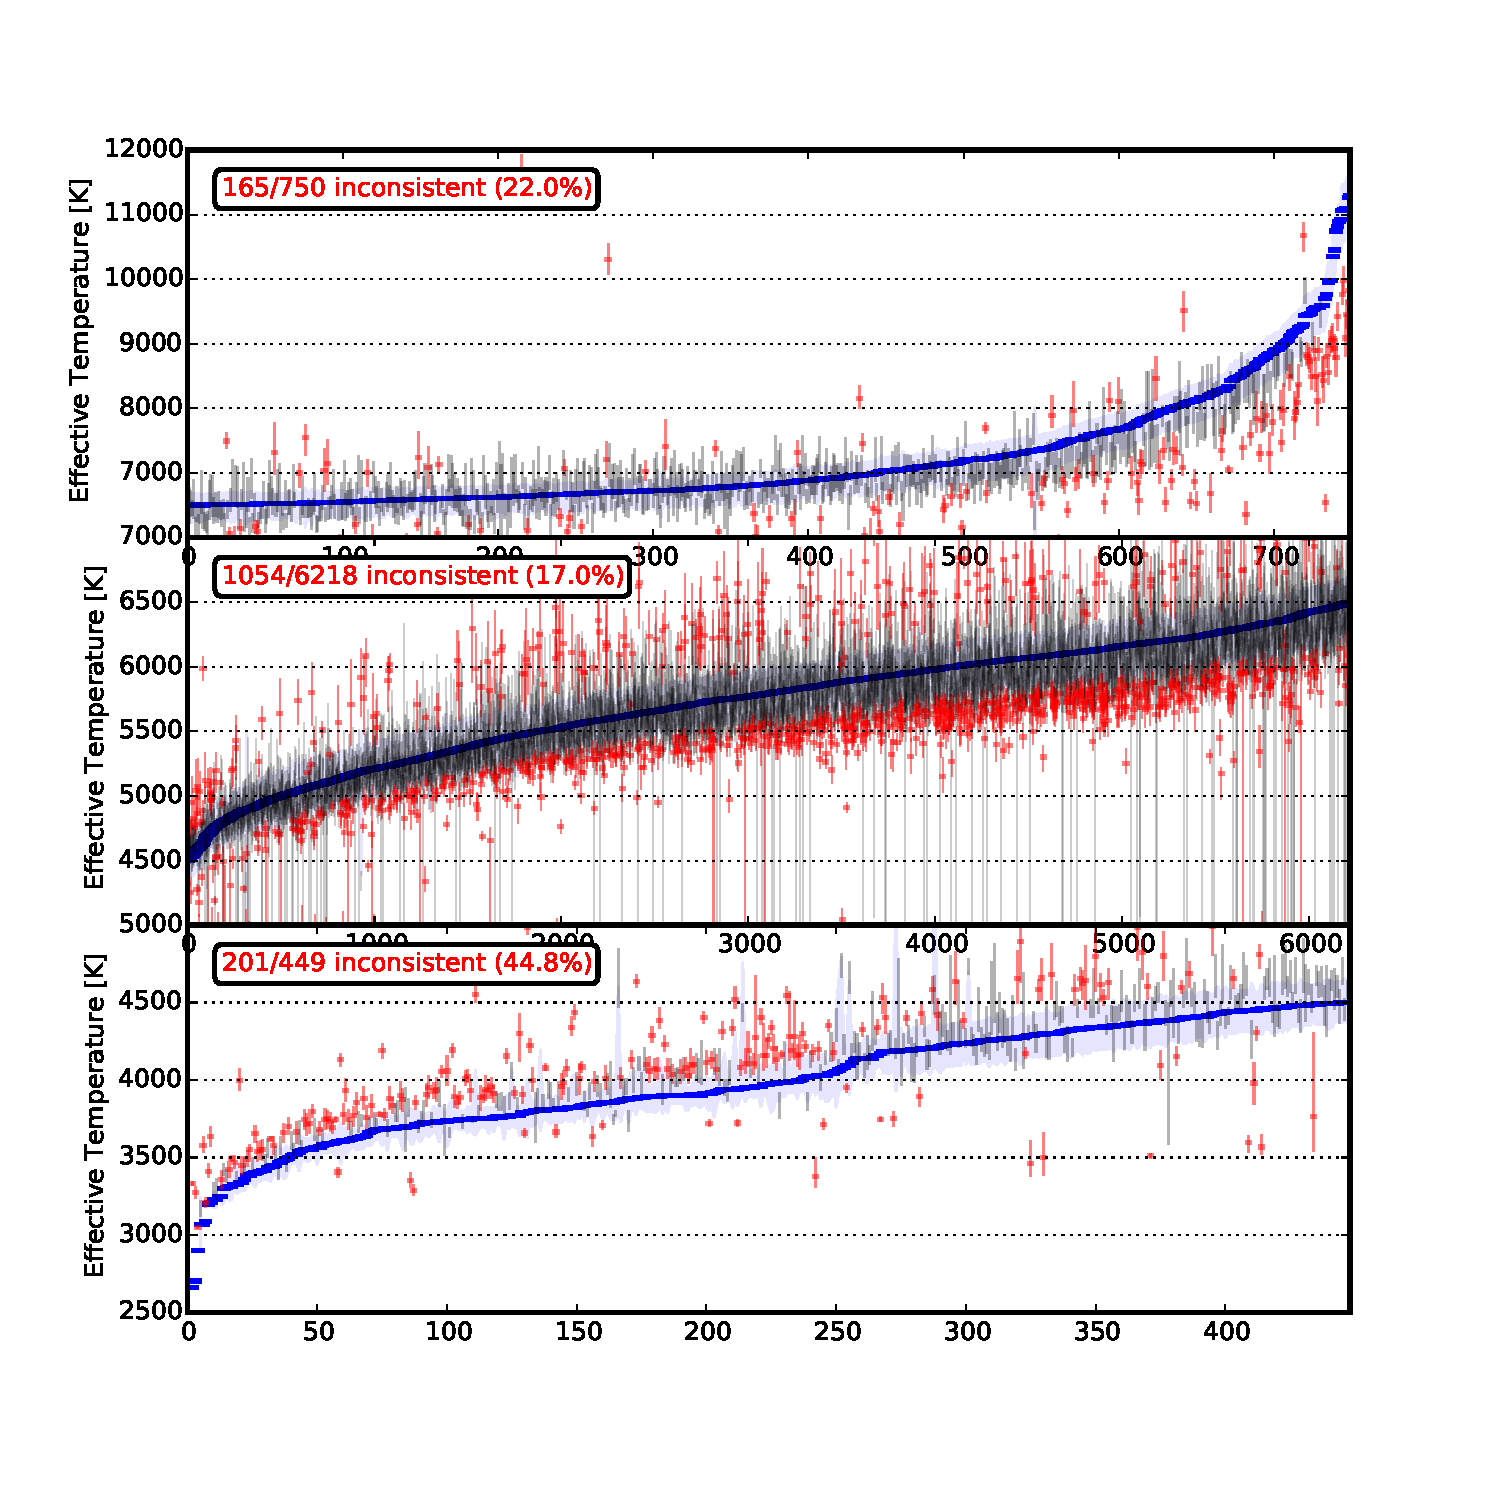
\includegraphics[width=7in]{figures/hubercompare_teff.pdf}
\end{center}
\caption{Comparison between effective temperatures estimated from the
  \isochrones\ analysis in this work and those from the
  \kepler\ stellar parameters catalog \citep[][hereafter
    \citetalias{Huber:2014}]{Huber:2014}.  Bottom panel shows stars
  for which \citetalias{Huber:2014} predicts $T_{\rm eff} < 4500$\,K,
  middle spans $4500\,{\rm K} < T_{\rm eff} < 6500\,{\rm K}$, and top
  has $T_{\rm eff} > 6500$\,K. Blue horizontal bold lines are the
  \citetalias{Huber:2014} values in sorted order; blue shading
  represents the error bars from \citetalias{Huber:2014}.  Vertical
  lines span the 1$\sigma$ credible region of the \isochrones\ fits;
  these lines are grey if they overlap with the
  \citetalias{Huber:2014} 1$\sigma$ region and red (with the median
  marked by a point) if they are inconsistent.  This comparison shows
  that the stellar parameters estimated in this work are broadly
  consistent with \citetalias{Huber:2014}, though less so for the
  coolest and hottest stars.
\figlabel{starsteff}}
\end{figure*}


\begin{figure*}[p]
\begin{center}
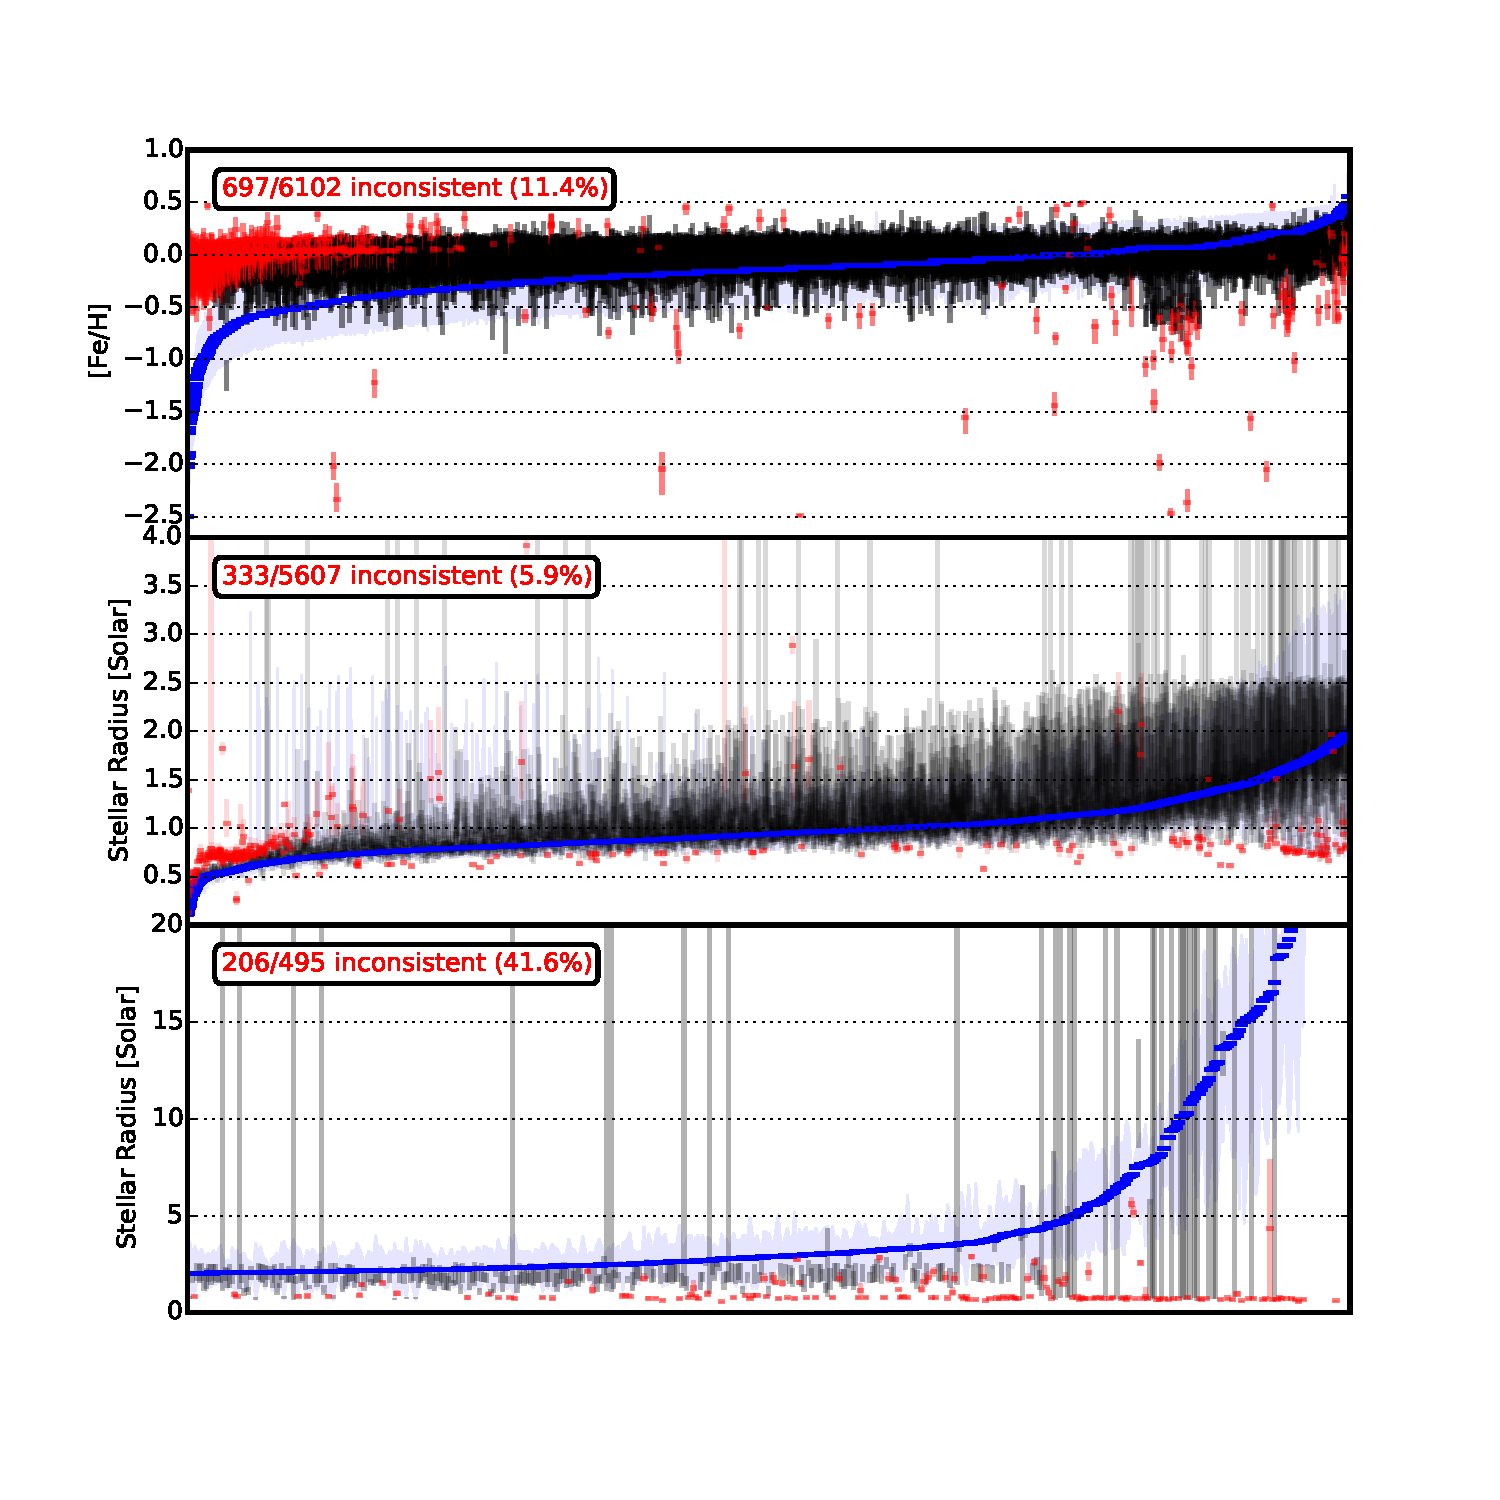
\includegraphics[width=7in]{figures/hubercompare_fehradius.pdf}
\end{center}
\caption{Comparison between metallicities and radii estimated from the
  \isochrones\ analysis in this work and those from the
  \kepler\ stellar parameters catalog \citep[][hereafter
    \citetalias{Huber:2014}]{Huber:2014}.  Top panel shows metallicity
  for all stars in the sample.  The middle panel shows stars for which
  \citetalias{Huber:2014} estimates $R_\star < 2\,R_\odot$, and the
  bottom shows $R_\star > 2\,R_\odot$. Blue horizontal bold lines are
  the \citetalias{Huber:2014} values in sorted order; blue shading
  represents the error bars from \citetalias{Huber:2014}.  Vertical
  lines span the 1$\sigma$ credible region of the \isochrones\ fits;
  these lines are grey if they overlap with the
  \citetalias{Huber:2014} 1$\sigma$ region and red (with the median
  marked by a point) if they are inconsistent.  This comparison shows
  that the stellar parameters estimated in this work are broadly
  consistent with \citetalias{Huber:2014}, though less so for the more
  evolved stars.  The metallicity estimates of the
  \isochrones\ calculations are driven by the use of the local
  metallicity prior \citep[][\tab{priors}]{Hayden:2015,
    Casagrande:2011}.
\figlabel{starsfehradius}}
\end{figure*}



\begin{figure*}[p]
\begin{center}
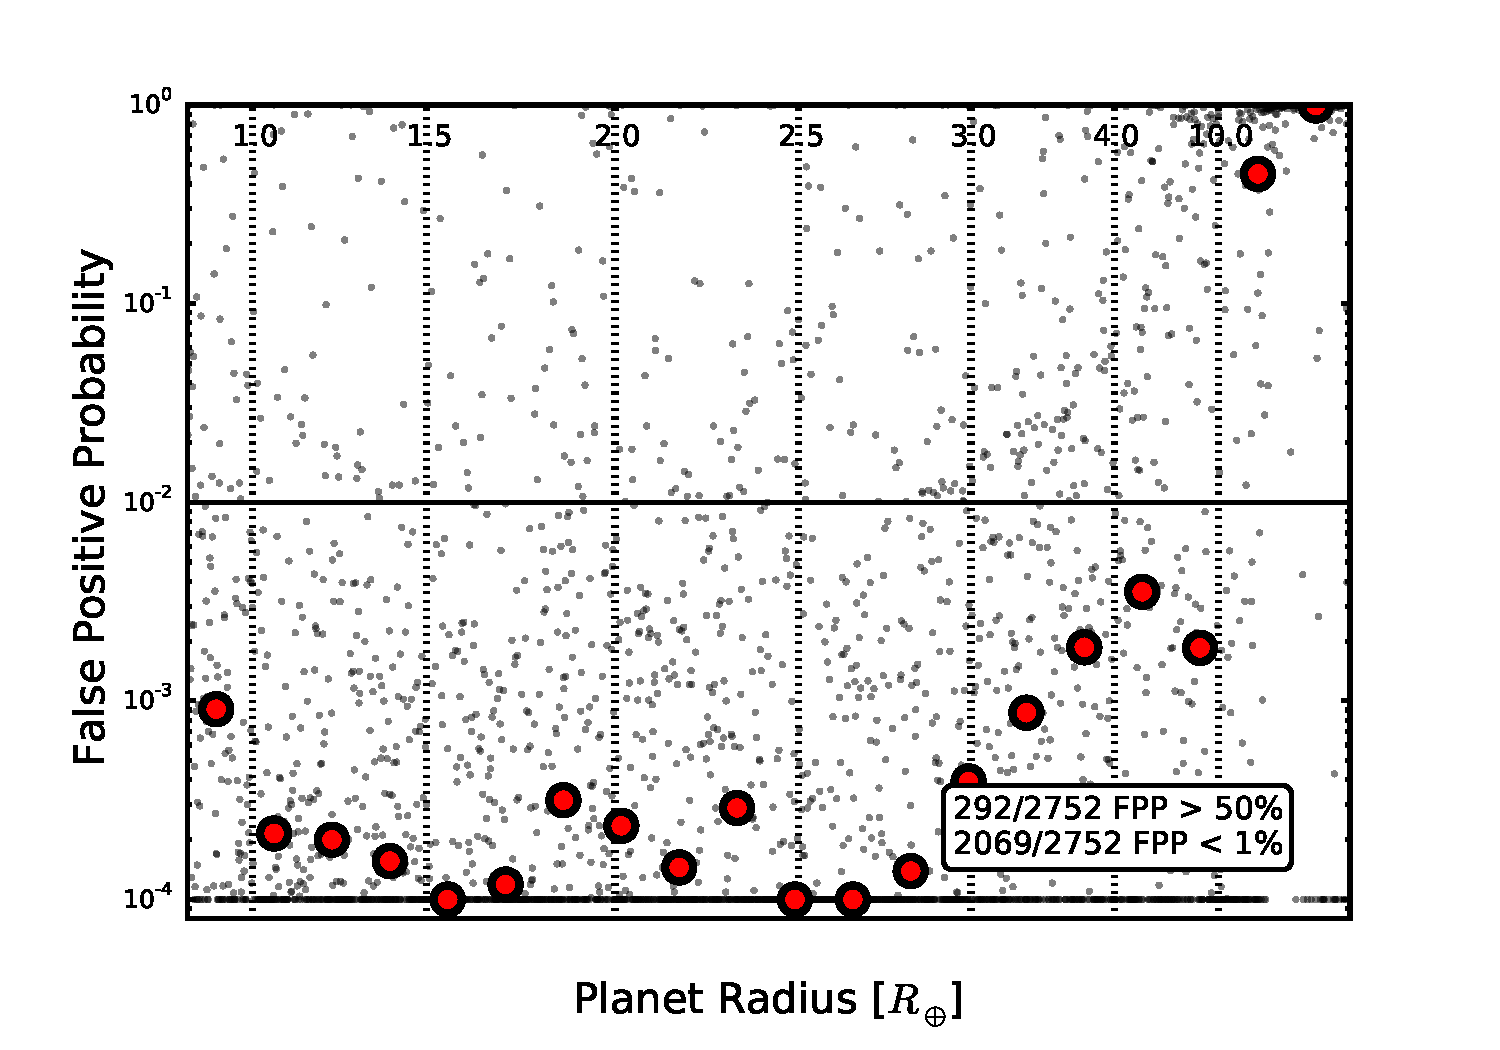
\includegraphics[width=7in]{figures/fpp_summary_all.pdf}
\end{center}
\caption{False positive probabilities of all CANDIDATE or CONFIRMED
  KOIs for which we consider the \vespa\ calculations to be reliable
  (floored at $10^{-4}$ for visualization purposes), meaning they are
  considered to be reliably located on the target star ($ {\rm Pr} >
  0.99$, with ``score'' $> \posprobthresh$) according to pixel-level analysis
  \citep{Bryson:KSCI}, and have $L_{\rm tot} > 10^{-3}$, indicating
  that the hypotheses tested by \vespa\ are not all poor explanations
  of the data (see \sect{results:fpp}).  Of these \nreliable\ KOIs,
  \nval\ have FPPs less than 1\% (\nvalnew\ of which have not yet been
  dispositioned as CONFIRMED).  Noteably, \nreliableFP\ are likely
  false positives (FPP $> 0.5$), consistent with the
  \citet{Morton:2011b} and \citet{Fressin:2013} \emph{a priori}
  estimates of the overall \kepler\ candidate false positive rate.
  \figlabel{fppall}}
\end{figure*}


\begin{figure*}[p]
\begin{center}
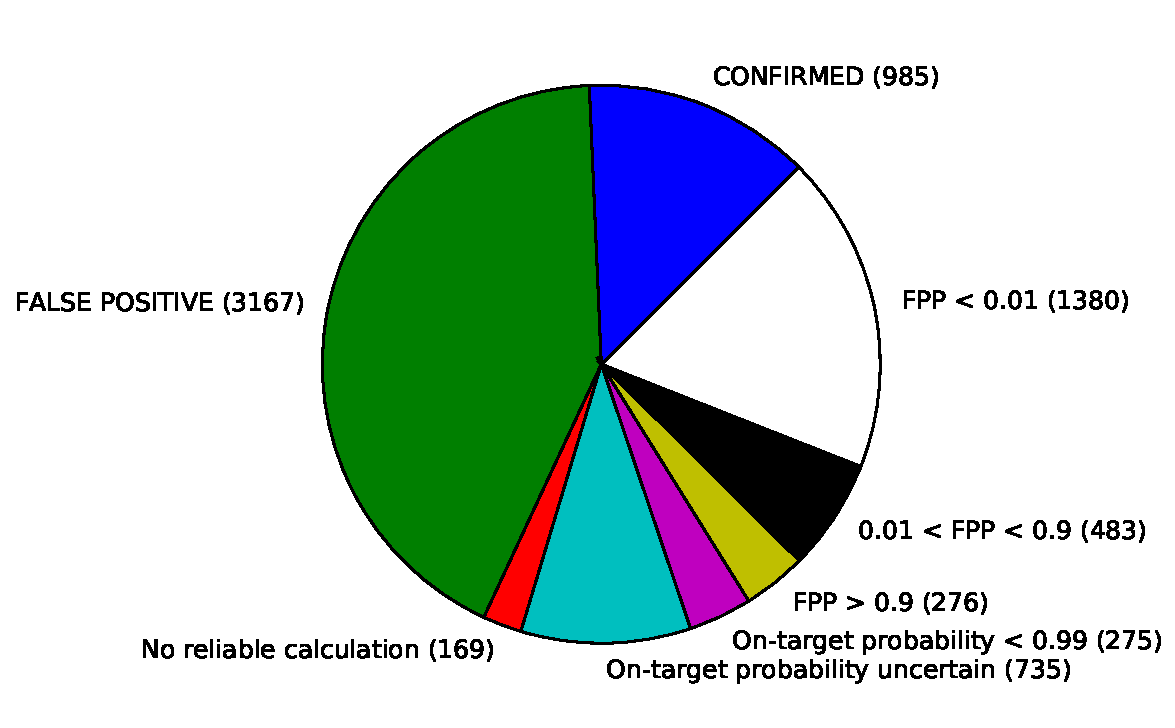
\includegraphics[width=7in]{figures/fpp_pie.pdf}
\end{center}
\caption{A summary of how the the calculations presented in this paper
  advance our understanding of the true nature of KOIs.  More than
  half of all KOIs to date have already been dispositioned FALSE
  POSITIVE or CONFIRMED.  Those dispositioned CANDIDATE we further
  categorize according to their reliability.  The ``no reliable
  calculation'' category means that either the \vespa\ calculation was
  not successful, or that $L_{\rm tot} < 10^{-3}$.  ``On-target
  probability uncertain'' indicates that the positional probability
  calculations of \citet{Bryson:KSCI} are not reliable (score $<
  \posprobthresh$).  ``On-target probability $<$ 0.99'' means that the positional
  probability calculations indicate that there is a non-negligible
  chance that the source of the transit signal is not at the position
  of the KOI.  The remaining three categories are all CANDIDATE KOIs
  reliably confirmed to be located at the presumed target star,
  grouped by false positive probability.  \nvalnew\ of these are new
  planet validations, and \nfpnew\ are new likely false positives.
  \figlabel{fpppie}}
\end{figure*}

\begin{figure*}[p]
\begin{center}
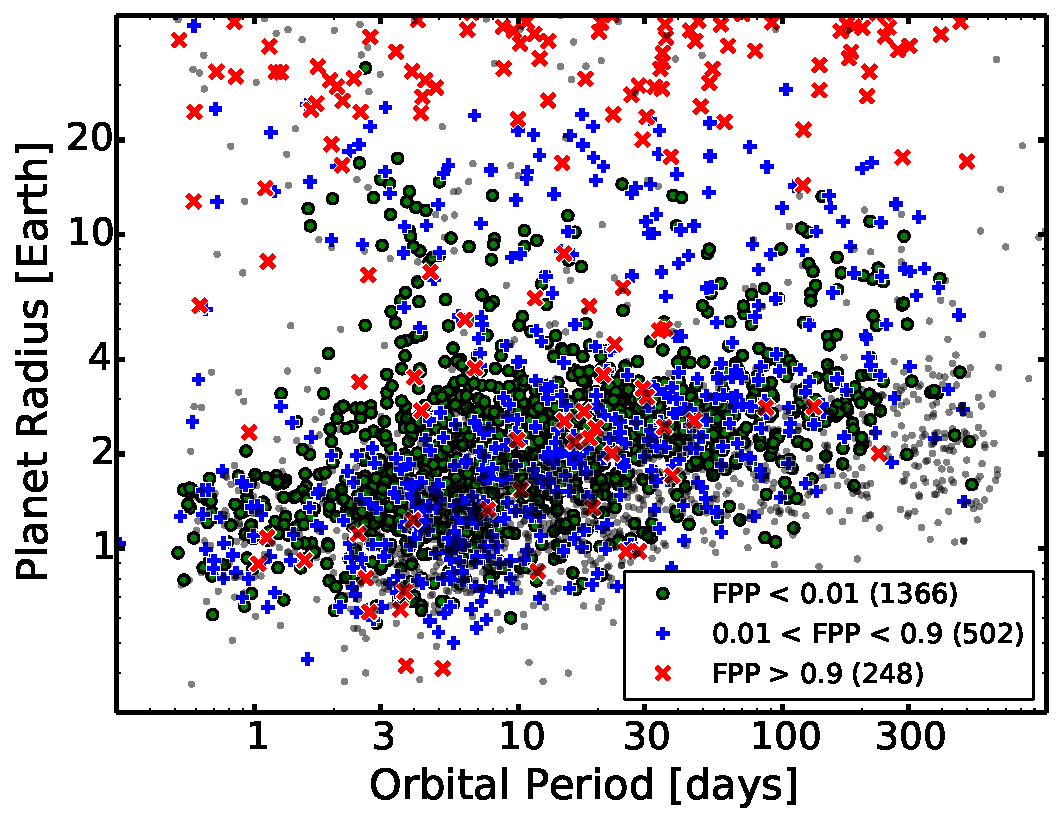
\includegraphics[width=7in]{figures/RP_cand.pdf}
\end{center}
\caption{Periods and radii of KOIs with CANDIDATE disposition, grouped
  by FPP value.  Green circles are most likely to be planets, red X's
  are most likely to be false positives, and blue plusses have
  intermediate FPPs.  Grey dots are KOIs for which the
  \vespa\ calculation is considered less reliable.  
  \figlabel{rpcand}}
\end{figure*}



%\capstartfalse

\begin{deluxetable*}{lccccccccccc}
\tablewidth{0pt}
\tabletypesize{\scriptsize}
\tablecaption{Stellar Properties
\tablabel{stars}}
\tablehead{\colhead{KOI} &
    \colhead{$M_\star$} &
    \colhead{$R_\star$} &
    \colhead{$T_{\rm eff}$} &
    \colhead{$\log g$} &
    \colhead{[Fe/H]} &
    \colhead{Age} &
    \colhead{$d$} &
    \colhead{$A_V$}&
    \colhead{$\pi\left(T_{\rm eff}\right)$} &
    \colhead{$\pi\left(\log g\right)$} &
    \colhead{$\pi\left({\rm [Fe/H]}\right)$} \\
    \colhead{} &
    \colhead{($M_\odot$)} &
    \colhead{($R_\odot$)} &
    \colhead{(K)} &
    \colhead{(cgs)} &
    \colhead{(dex)} &
    \colhead{(Gyr)} &
    \colhead{(pc)} &
    \colhead{(mag)} &
    \colhead{} &
    \colhead{} &
    \colhead{} 
    }
\startdata
K00757.03 &${ 0.80 }^{ +0.04 }_{ -0.04 }$&${ 0.76 }^{ +0.03 }_{ -0.04 }$&${ 5017 }^{ +54 }_{ -57 }$&${ 4.59 }^{ +0.03 }_{ -0.05 }$&${ -0.04 }^{ +0.15 }_{ -0.17 }$&${ 9.69 }^{ +0.37 }_{ -0.41 }$&${ 879 }^{ +42 }_{ -49 }$&${ 0.10 }^{ +0.06 }_{ -0.06 }$&--&--&--\\ 
K00758.01 &${ 0.79 }^{ +0.04 }_{ -0.04 }$&${ 0.74 }^{ +0.03 }_{ -0.04 }$&${ 4913 }^{ +94 }_{ -87 }$&${ 4.60 }^{ +0.02 }_{ -0.04 }$&${ -0.03 }^{ +0.15 }_{ -0.17 }$&${ 9.67 }^{ +0.36 }_{ -0.38 }$&${ 651 }^{ +32 }_{ -37 }$&${ 0.17 }^{ +0.12 }_{ -0.11 }$&--&--&--\\ 
K00759.02 &${ 0.84 }^{ +0.05 }_{ -0.05 }$&${ 0.81 }^{ +0.06 }_{ -0.06 }$&${ 5328 }^{ +60 }_{ -55 }$&${ 4.56 }^{ +0.04 }_{ -0.08 }$&${ -0.14 }^{ +0.16 }_{ -0.19 }$&${ 9.64 }^{ +0.39 }_{ -0.43 }$&${ 775 }^{ +64 }_{ -61 }$&${ 0.06 }^{ +0.05 }_{ -0.04 }$&--&--&--\\ 
K00760.01 &${ 1.06 }^{ +0.07 }_{ -0.06 }$&${ 1.07 }^{ +0.25 }_{ -0.10 }$&${ 5895 }^{ +86 }_{ -102 }$&${ 4.40 }^{ +0.08 }_{ -0.17 }$&${ 0.06 }^{ +0.15 }_{ -0.15 }$&${ 9.59 }^{ +0.20 }_{ -0.35 }$&${ 1356 }^{ +311 }_{ -141 }$&${ 0.14 }^{ +0.05 }_{ -0.08 }$&--&--&--\\ 
K00761.01 &${ 0.94 }^{ +0.04 }_{ -0.04 }$&${ 0.92 }^{ +0.19 }_{ -0.06 }$&${ 5505 }^{ +69 }_{ -90 }$&${ 4.49 }^{ +0.05 }_{ -0.17 }$&${ 0.09 }^{ +0.13 }_{ -0.13 }$&${ 9.71 }^{ +0.35 }_{ -0.46 }$&${ 1051 }^{ +223 }_{ -75 }$&${ 0.32 }^{ +0.04 }_{ -0.09 }$&--&--&--\\ 
K00762.01 &${ 1.03 }^{ +0.09 }_{ -0.08 }$&${ 1.05 }^{ +0.25 }_{ -0.12 }$&${ 5887 }^{ +165 }_{ -179 }$&${ 4.41 }^{ +0.09 }_{ -0.17 }$&${ 0.01 }^{ +0.14 }_{ -0.17 }$&${ 9.58 }^{ +0.24 }_{ -0.34 }$&${ 1330 }^{ +317 }_{ -168 }$&${ 0.28 }^{ +0.12 }_{ -0.15 }$&--&--&--\\ 
K00763.01 &${ 0.99 }^{ +0.04 }_{ -0.05 }$&${ 0.98 }^{ +0.18 }_{ -0.08 }$&${ 5710 }^{ +73 }_{ -91 }$&${ 4.45 }^{ +0.06 }_{ -0.15 }$&${ 0.05 }^{ +0.14 }_{ -0.17 }$&${ 9.67 }^{ +0.27 }_{ -0.39 }$&${ 1304 }^{ +241 }_{ -109 }$&${ 0.15 }^{ +0.04 }_{ -0.08 }$&--&--&--\\ 
K00764.01 &${ 0.91 }^{ +0.04 }_{ -0.04 }$&${ 0.87 }^{ +0.07 }_{ -0.05 }$&${ 5327 }^{ +53 }_{ -70 }$&${ 4.53 }^{ +0.04 }_{ -0.09 }$&${ 0.15 }^{ +0.15 }_{ -0.16 }$&${ 9.67 }^{ +0.37 }_{ -0.44 }$&${ 907 }^{ +76 }_{ -52 }$&${ 0.21 }^{ +0.03 }_{ -0.07 }$&--&--&--\\ 
K00765.01 &${ 0.87 }^{ +0.04 }_{ -0.05 }$&${ 0.82 }^{ +0.06 }_{ -0.05 }$&${ 5352 }^{ +61 }_{ -61 }$&${ 4.55 }^{ +0.03 }_{ -0.07 }$&${ -0.06 }^{ +0.15 }_{ -0.17 }$&${ 9.59 }^{ +0.40 }_{ -0.40 }$&${ 877 }^{ +70 }_{ -59 }$&${ 0.09 }^{ +0.05 }_{ -0.06 }$&--&--&--\\ 
K00766.01 &${ 1.15 }^{ +0.10 }_{ -0.07 }$&${ 1.20 }^{ +0.32 }_{ -0.13 }$&${ 6038 }^{ +98 }_{ -109 }$&${ 4.34 }^{ +0.08 }_{ -0.18 }$&${ 0.14 }^{ +0.15 }_{ -0.14 }$&${ 9.50 }^{ +0.15 }_{ -0.29 }$&${ 1778 }^{ +463 }_{ -208 }$&${ 0.14 }^{ +0.05 }_{ -0.08 }$&--&--&--\\ 
K00767.01 &${ 0.99 }^{ +0.05 }_{ -0.06 }$&${ 0.99 }^{ +0.22 }_{ -0.09 }$&${ 5709 }^{ +89 }_{ -134 }$&${ 4.44 }^{ +0.07 }_{ -0.17 }$&${ 0.07 }^{ +0.14 }_{ -0.15 }$&${ 9.68 }^{ +0.25 }_{ -0.41 }$&${ 980 }^{ +218 }_{ -98 }$&${ 0.36 }^{ +0.06 }_{ -0.12 }$&--&--&--\\ 
K00768.01 &${ 0.81 }^{ +0.03 }_{ -0.04 }$&${ 0.77 }^{ +0.03 }_{ -0.03 }$&${ 5035 }^{ +47 }_{ -49 }$&${ 4.58 }^{ +0.02 }_{ -0.05 }$&${ 0.00 }^{ +0.13 }_{ -0.15 }$&${ 9.68 }^{ +0.36 }_{ -0.40 }$&${ 857 }^{ +38 }_{ -39 }$&${ 0.08 }^{ +0.05 }_{ -0.06 }$&--&--&--\\ 
K00769.01 &${ 0.97 }^{ +0.05 }_{ -0.04 }$&${ 0.95 }^{ +0.17 }_{ -0.06 }$&${ 5624 }^{ +75 }_{ -91 }$&${ 4.47 }^{ +0.05 }_{ -0.15 }$&${ 0.08 }^{ +0.15 }_{ -0.14 }$&${ 9.65 }^{ +0.32 }_{ -0.43 }$&${ 1139 }^{ +200 }_{ -87 }$&${ 0.15 }^{ +0.05 }_{ -0.08 }$&--&--&--\\ 
K00770.01 &${ 0.93 }^{ +0.04 }_{ -0.05 }$&${ 0.89 }^{ +0.10 }_{ -0.06 }$&${ 5565 }^{ +88 }_{ -106 }$&${ 4.51 }^{ +0.04 }_{ -0.10 }$&${ -0.02 }^{ +0.15 }_{ -0.17 }$&${ 9.63 }^{ +0.33 }_{ -0.41 }$&${ 1114 }^{ +127 }_{ -77 }$&${ 0.16 }^{ +0.07 }_{ -0.10 }$&--&--&--\\ 
K00772.01 &${ 1.05 }^{ +0.06 }_{ -0.06 }$&${ 1.05 }^{ +0.21 }_{ -0.09 }$&${ 5917 }^{ +100 }_{ -85 }$&${ 4.41 }^{ +0.07 }_{ -0.14 }$&${ 0.01 }^{ +0.13 }_{ -0.17 }$&${ 9.56 }^{ +0.22 }_{ -0.32 }$&${ 1369 }^{ +274 }_{ -127 }$&${ 0.09 }^{ +0.07 }_{ -0.06 }$&--&--&--\\ 
K00773.01 &${ 0.95 }^{ +0.04 }_{ -0.05 }$&${ 0.92 }^{ +0.11 }_{ -0.06 }$&${ 5627 }^{ +75 }_{ -80 }$&${ 4.50 }^{ +0.05 }_{ -0.11 }$&${ -0.01 }^{ +0.15 }_{ -0.18 }$&${ 9.61 }^{ +0.33 }_{ -0.39 }$&${ 1011 }^{ +128 }_{ -74 }$&${ 0.12 }^{ +0.05 }_{ -0.07 }$&--&--&--\\ 
K00774.01 &${ 0.97 }^{ +0.06 }_{ -0.07 }$&${ 0.96 }^{ +0.16 }_{ -0.09 }$&${ 5760 }^{ +109 }_{ -104 }$&${ 4.46 }^{ +0.07 }_{ -0.13 }$&${ -0.07 }^{ +0.15 }_{ -0.21 }$&${ 9.65 }^{ +0.27 }_{ -0.40 }$&${ 1170 }^{ +189 }_{ -113 }$&${ 0.12 }^{ +0.08 }_{ -0.08 }$&--&--&--\\ 
K00775.01 &${ 0.66 }^{ +0.02 }_{ -0.03 }$&${ 0.63 }^{ +0.02 }_{ -0.02 }$&${ 4242 }^{ +42 }_{ -36 }$&${ 4.66 }^{ +0.01 }_{ -0.02 }$&${ -0.00 }^{ +0.12 }_{ -0.09 }$&${ 9.55 }^{ +0.36 }_{ -0.35 }$&${ 336 }^{ +12 }_{ -15 }$&${ 0.05 }^{ +0.06 }_{ -0.03 }$&(4117, 92)&(4.66, 0.03)&(0.04, 0.14)\\ 
K00775.02 &${ 0.66 }^{ +0.02 }_{ -0.03 }$&${ 0.63 }^{ +0.02 }_{ -0.02 }$&${ 4241 }^{ +42 }_{ -37 }$&${ 4.66 }^{ +0.01 }_{ -0.02 }$&${ -0.00 }^{ +0.11 }_{ -0.09 }$&${ 9.54 }^{ +0.37 }_{ -0.32 }$&${ 336 }^{ +12 }_{ -15 }$&${ 0.04 }^{ +0.06 }_{ -0.03 }$&(4117, 92)&(4.66, 0.03)&(0.04, 0.14)\\ 
K00775.03 &${ 0.66 }^{ +0.02 }_{ -0.03 }$&${ 0.63 }^{ +0.02 }_{ -0.02 }$&${ 4241 }^{ +40 }_{ -34 }$&${ 4.66 }^{ +0.01 }_{ -0.02 }$&${ -0.01 }^{ +0.11 }_{ -0.09 }$&${ 9.53 }^{ +0.37 }_{ -0.32 }$&${ 336 }^{ +11 }_{ -14 }$&${ 0.04 }^{ +0.06 }_{ -0.03 }$&(4117, 92)&(4.66, 0.03)&(0.04, 0.14)\\ 
K00776.01 &${ 0.88 }^{ +0.04 }_{ -0.05 }$&${ 0.84 }^{ +0.07 }_{ -0.05 }$&${ 5355 }^{ +60 }_{ -72 }$&${ 4.54 }^{ +0.04 }_{ -0.08 }$&${ 0.00 }^{ +0.15 }_{ -0.17 }$&${ 9.65 }^{ +0.38 }_{ -0.42 }$&${ 978 }^{ +80 }_{ -65 }$&${ 0.14 }^{ +0.04 }_{ -0.08 }$&--&--&--\\ 
K00777.01 &${ 0.82 }^{ +0.04 }_{ -0.05 }$&${ 0.79 }^{ +0.05 }_{ -0.05 }$&${ 5195 }^{ +56 }_{ -71 }$&${ 4.57 }^{ +0.04 }_{ -0.07 }$&${ -0.08 }^{ +0.16 }_{ -0.20 }$&${ 9.69 }^{ +0.36 }_{ -0.41 }$&${ 817 }^{ +57 }_{ -60 }$&${ 0.17 }^{ +0.04 }_{ -0.08 }$&--&--&--\\ 
K00778.01 &${ 0.60 }^{ +0.04 }_{ -0.03 }$&${ 0.57 }^{ +0.03 }_{ -0.02 }$&${ 4192 }^{ +41 }_{ -43 }$&${ 4.69 }^{ +0.01 }_{ -0.02 }$&${ -0.27 }^{ +0.14 }_{ -0.14 }$&${ 9.52 }^{ +0.42 }_{ -0.33 }$&${ 302 }^{ +19 }_{ -18 }$&${ 0.06 }^{ +0.05 }_{ -0.04 }$&(4128, 100)&(4.70, 0.02)&(-0.36, 0.16)\\ 
K00779.01 &${ 0.97 }^{ +0.04 }_{ -0.05 }$&${ 0.95 }^{ +0.15 }_{ -0.07 }$&${ 5652 }^{ +83 }_{ -102 }$&${ 4.47 }^{ +0.06 }_{ -0.14 }$&${ 0.03 }^{ +0.13 }_{ -0.16 }$&${ 9.67 }^{ +0.29 }_{ -0.42 }$&${ 1233 }^{ +200 }_{ -100 }$&${ 0.20 }^{ +0.05 }_{ -0.09 }$&--&--&--\\ 
K00780.01 &${ 0.79 }^{ +0.04 }_{ -0.05 }$&${ 0.75 }^{ +0.03 }_{ -0.04 }$&${ 4945 }^{ +70 }_{ -71 }$&${ 4.60 }^{ +0.03 }_{ -0.04 }$&${ -0.05 }^{ +0.15 }_{ -0.18 }$&${ 9.67 }^{ +0.36 }_{ -0.39 }$&${ 651 }^{ +32 }_{ -38 }$&${ 0.14 }^{ +0.09 }_{ -0.09 }$&--&--&--\\ 
K00780.02 &${ 0.79 }^{ +0.04 }_{ -0.04 }$&${ 0.75 }^{ +0.03 }_{ -0.04 }$&${ 4944 }^{ +74 }_{ -71 }$&${ 4.60 }^{ +0.02 }_{ -0.04 }$&${ -0.05 }^{ +0.15 }_{ -0.17 }$&${ 9.66 }^{ +0.37 }_{ -0.39 }$&${ 651 }^{ +30 }_{ -36 }$&${ 0.14 }^{ +0.09 }_{ -0.09 }$&--&--&--\\ 
K00781.01 &${ 0.51 }^{ +0.02 }_{ -0.03 }$&${ 0.49 }^{ +0.02 }_{ -0.03 }$&${ 3701 }^{ +39 }_{ -40 }$&${ 4.77 }^{ +0.02 }_{ -0.02 }$&${ -0.02 }^{ +0.09 }_{ -0.09 }$&${ 9.63 }^{ +0.38 }_{ -0.39 }$&${ 243 }^{ +15 }_{ -17 }$&${ 0.14 }^{ +0.08 }_{ -0.08 }$&(3648, 65)&(4.79, 0.06)&(0.00, 0.14)\\ 
K00782.01 &${ 1.00 }^{ +0.05 }_{ -0.05 }$&${ 0.99 }^{ +0.21 }_{ -0.08 }$&${ 5723 }^{ +69 }_{ -88 }$&${ 4.45 }^{ +0.06 }_{ -0.16 }$&${ 0.06 }^{ +0.14 }_{ -0.16 }$&${ 9.66 }^{ +0.26 }_{ -0.41 }$&${ 1180 }^{ +253 }_{ -99 }$&${ 0.17 }^{ +0.04 }_{ -0.07 }$&--&--&--\\ 
K00783.01 &${ 0.94 }^{ +0.04 }_{ -0.05 }$&${ 0.91 }^{ +0.12 }_{ -0.06 }$&${ 5520 }^{ +73 }_{ -108 }$&${ 4.50 }^{ +0.05 }_{ -0.12 }$&${ 0.07 }^{ +0.16 }_{ -0.15 }$&${ 9.65 }^{ +0.35 }_{ -0.43 }$&${ 875 }^{ +113 }_{ -61 }$&${ 0.27 }^{ +0.05 }_{ -0.10 }$&--&--&--\\ 
K00784.01 &${ 0.59 }^{ +0.03 }_{ -0.04 }$&${ 0.57 }^{ +0.03 }_{ -0.03 }$&${ 4147 }^{ +45 }_{ -45 }$&${ 4.70 }^{ +0.02 }_{ -0.02 }$&${ -0.26 }^{ +0.13 }_{ -0.14 }$&${ 9.54 }^{ +0.38 }_{ -0.33 }$&${ 325 }^{ +19 }_{ -21 }$&${ 0.04 }^{ +0.06 }_{ -0.03 }$&(4059, 93)&(4.70, 0.02)&(-0.26, 0.18)\\ 
K00784.02 &${ 0.59 }^{ +0.03 }_{ -0.04 }$&${ 0.57 }^{ +0.03 }_{ -0.03 }$&${ 4147 }^{ +47 }_{ -46 }$&${ 4.70 }^{ +0.02 }_{ -0.02 }$&${ -0.26 }^{ +0.12 }_{ -0.14 }$&${ 9.53 }^{ +0.39 }_{ -0.32 }$&${ 325 }^{ +20 }_{ -22 }$&${ 0.05 }^{ +0.06 }_{ -0.03 }$&(4059, 93)&(4.70, 0.02)&(-0.26, 0.18)\\ 
K00785.01 &${ 0.87 }^{ +0.05 }_{ -0.05 }$&${ 0.84 }^{ +0.07 }_{ -0.06 }$&${ 5403 }^{ +97 }_{ -106 }$&${ 4.54 }^{ +0.04 }_{ -0.09 }$&${ -0.09 }^{ +0.16 }_{ -0.19 }$&${ 9.65 }^{ +0.38 }_{ -0.45 }$&${ 968 }^{ +90 }_{ -76 }$&${ 0.17 }^{ +0.09 }_{ -0.11 }$&--&--&--\\ 
K00786.01 &${ 1.08 }^{ +0.10 }_{ -0.06 }$&${ 1.11 }^{ +0.38 }_{ -0.11 }$&${ 5890 }^{ +77 }_{ -99 }$&${ 4.38 }^{ +0.08 }_{ -0.22 }$&${ 0.13 }^{ +0.15 }_{ -0.15 }$&${ 9.57 }^{ +0.18 }_{ -0.34 }$&${ 1342 }^{ +446 }_{ -145 }$&${ 0.21 }^{ +0.04 }_{ -0.08 }$&--&--&--\\ 
K00787.01 &${ 0.97 }^{ +0.06 }_{ -0.05 }$&${ 0.95 }^{ +0.20 }_{ -0.07 }$&${ 5654 }^{ +118 }_{ -108 }$&${ 4.47 }^{ +0.06 }_{ -0.16 }$&${ 0.03 }^{ +0.13 }_{ -0.16 }$&${ 9.65 }^{ +0.28 }_{ -0.40 }$&${ 1155 }^{ +238 }_{ -99 }$&${ 0.15 }^{ +0.10 }_{ -0.10 }$&--&--&--\\ 
K00787.02 &${ 0.96 }^{ +0.05 }_{ -0.05 }$&${ 0.94 }^{ +0.15 }_{ -0.07 }$&${ 5647 }^{ +123 }_{ -112 }$&${ 4.48 }^{ +0.05 }_{ -0.13 }$&${ 0.02 }^{ +0.13 }_{ -0.17 }$&${ 9.61 }^{ +0.32 }_{ -0.39 }$&${ 1142 }^{ +181 }_{ -93 }$&${ 0.15 }^{ +0.10 }_{ -0.10 }$&--&--&--\\ 
K00788.01 &${ 0.80 }^{ +0.04 }_{ -0.05 }$&${ 0.76 }^{ +0.03 }_{ -0.04 }$&${ 5021 }^{ +64 }_{ -62 }$&${ 4.58 }^{ +0.03 }_{ -0.04 }$&${ -0.04 }^{ +0.15 }_{ -0.16 }$&${ 9.70 }^{ +0.33 }_{ -0.39 }$&${ 666 }^{ +33 }_{ -37 }$&${ 0.11 }^{ +0.07 }_{ -0.08 }$&--&--&--\\ 
K00790.01 &${ 0.84 }^{ +0.04 }_{ -0.05 }$&${ 0.80 }^{ +0.06 }_{ -0.05 }$&${ 5261 }^{ +93 }_{ -81 }$&${ 4.56 }^{ +0.04 }_{ -0.07 }$&${ -0.09 }^{ +0.15 }_{ -0.18 }$&${ 9.67 }^{ +0.37 }_{ -0.44 }$&${ 825 }^{ +60 }_{ -60 }$&${ 0.12 }^{ +0.09 }_{ -0.08 }$&--&--&--\\ 
K00790.02 &${ 0.84 }^{ +0.04 }_{ -0.05 }$&${ 0.80 }^{ +0.05 }_{ -0.05 }$&${ 5257 }^{ +93 }_{ -74 }$&${ 4.56 }^{ +0.04 }_{ -0.07 }$&${ -0.09 }^{ +0.15 }_{ -0.18 }$&${ 9.65 }^{ +0.38 }_{ -0.42 }$&${ 823 }^{ +59 }_{ -58 }$&${ 0.11 }^{ +0.10 }_{ -0.08 }$&--&--&--\\ 
K00791.01 &${ 0.92 }^{ +0.04 }_{ -0.05 }$&${ 0.89 }^{ +0.09 }_{ -0.06 }$&${ 5559 }^{ +85 }_{ -82 }$&${ 4.51 }^{ +0.04 }_{ -0.10 }$&${ -0.05 }^{ +0.14 }_{ -0.17 }$&${ 9.60 }^{ +0.36 }_{ -0.39 }$&${ 951 }^{ +101 }_{ -68 }$&${ 0.10 }^{ +0.07 }_{ -0.07 }$&--&--&--\\ 
K00792.01 &${ 1.02 }^{ +0.09 }_{ -0.07 }$&${ 1.04 }^{ +0.21 }_{ -0.11 }$&${ 5908 }^{ +172 }_{ -172 }$&${ 4.42 }^{ +0.08 }_{ -0.14 }$&${ -0.03 }^{ +0.14 }_{ -0.18 }$&${ 9.58 }^{ +0.21 }_{ -0.32 }$&${ 1190 }^{ +245 }_{ -137 }$&${ 0.22 }^{ +0.13 }_{ -0.14 }$&--&--&--\\ 
K00793.01 &${ 1.12 }^{ +0.11 }_{ -0.09 }$&${ 1.17 }^{ +0.37 }_{ -0.15 }$&${ 6033 }^{ +119 }_{ -187 }$&${ 4.35 }^{ +0.10 }_{ -0.20 }$&${ 0.09 }^{ +0.14 }_{ -0.14 }$&${ 9.53 }^{ +0.18 }_{ -0.29 }$&${ 1257 }^{ +396 }_{ -168 }$&${ 0.46 }^{ +0.07 }_{ -0.14 }$&--&--&--\\ 
K00794.01 &${ 0.96 }^{ +0.06 }_{ -0.06 }$&${ 0.95 }^{ +0.16 }_{ -0.08 }$&${ 5703 }^{ +141 }_{ -149 }$&${ 4.47 }^{ +0.06 }_{ -0.13 }$&${ -0.03 }^{ +0.14 }_{ -0.18 }$&${ 9.64 }^{ +0.29 }_{ -0.38 }$&${ 976 }^{ +167 }_{ -94 }$&${ 0.23 }^{ +0.11 }_{ -0.13 }$&--&--&--\\ 
K00795.01 &${ 0.89 }^{ +0.06 }_{ -0.06 }$&${ 0.86 }^{ +0.08 }_{ -0.07 }$&${ 5493 }^{ +124 }_{ -119 }$&${ 4.53 }^{ +0.05 }_{ -0.09 }$&${ -0.11 }^{ +0.16 }_{ -0.19 }$&${ 9.64 }^{ +0.36 }_{ -0.43 }$&${ 1066 }^{ +98 }_{ -93 }$&${ 0.18 }^{ +0.11 }_{ -0.11 }$&--&--&--\\ 
K00796.01 &${ 0.80 }^{ +0.05 }_{ -0.06 }$&${ 0.76 }^{ +0.05 }_{ -0.06 }$&${ 5132 }^{ +107 }_{ -87 }$&${ 4.58 }^{ +0.04 }_{ -0.05 }$&${ -0.15 }^{ +0.16 }_{ -0.21 }$&${ 9.69 }^{ +0.36 }_{ -0.40 }$&${ 879 }^{ +60 }_{ -76 }$&${ 0.15 }^{ +0.12 }_{ -0.10 }$&--&--&--\\ 
K00797.01 &${ 0.93 }^{ +0.05 }_{ -0.06 }$&${ 0.90 }^{ +0.10 }_{ -0.07 }$&${ 5613 }^{ +112 }_{ -134 }$&${ 4.51 }^{ +0.05 }_{ -0.10 }$&${ -0.08 }^{ +0.15 }_{ -0.19 }$&${ 9.61 }^{ +0.33 }_{ -0.39 }$&${ 1190 }^{ +137 }_{ -100 }$&${ 0.21 }^{ +0.09 }_{ -0.12 }$&--&--&--\\ 
K00798.01 &${ 0.89 }^{ +0.04 }_{ -0.04 }$&${ 0.85 }^{ +0.08 }_{ -0.05 }$&${ 5342 }^{ +68 }_{ -105 }$&${ 4.53 }^{ +0.04 }_{ -0.09 }$&${ 0.07 }^{ +0.15 }_{ -0.14 }$&${ 9.68 }^{ +0.37 }_{ -0.44 }$&${ 950 }^{ +88 }_{ -58 }$&${ 0.34 }^{ +0.05 }_{ -0.11 }$&--&--&--\\ 
K00800.01 &${ 1.11 }^{ +0.08 }_{ -0.07 }$&${ 1.15 }^{ +0.31 }_{ -0.12 }$&${ 6003 }^{ +99 }_{ -137 }$&${ 4.36 }^{ +0.08 }_{ -0.18 }$&${ 0.09 }^{ +0.15 }_{ -0.16 }$&${ 9.54 }^{ +0.16 }_{ -0.31 }$&${ 1651 }^{ +438 }_{ -192 }$&${ 0.23 }^{ +0.05 }_{ -0.11 }$&--&--&--\\ 
K00800.02 &${ 1.11 }^{ +0.09 }_{ -0.07 }$&${ 1.15 }^{ +0.29 }_{ -0.13 }$&${ 6005 }^{ +102 }_{ -134 }$&${ 4.37 }^{ +0.08 }_{ -0.17 }$&${ 0.09 }^{ +0.15 }_{ -0.15 }$&${ 9.52 }^{ +0.18 }_{ -0.30 }$&${ 1651 }^{ +404 }_{ -190 }$&${ 0.23 }^{ +0.06 }_{ -0.11 }$&--&--&--\\ 
K00801.01 &${ 1.11 }^{ +0.11 }_{ -0.07 }$&${ 1.16 }^{ +0.33 }_{ -0.13 }$&${ 5963 }^{ +94 }_{ -126 }$&${ 4.36 }^{ +0.09 }_{ -0.19 }$&${ 0.15 }^{ +0.14 }_{ -0.15 }$&${ 9.53 }^{ +0.17 }_{ -0.32 }$&${ 1145 }^{ +327 }_{ -137 }$&${ 0.53 }^{ +0.05 }_{ -0.10 }$&--&--&--\\ 
K00802.01 &${ 0.96 }^{ +0.09 }_{ -0.07 }$&${ 0.95 }^{ +0.17 }_{ -0.09 }$&${ 5731 }^{ +255 }_{ -188 }$&${ 4.47 }^{ +0.07 }_{ -0.12 }$&${ -0.06 }^{ +0.15 }_{ -0.19 }$&${ 9.57 }^{ +0.30 }_{ -0.35 }$&${ 1247 }^{ +237 }_{ -130 }$&${ 0.24 }^{ +0.21 }_{ -0.16 }$&--&--&--
\enddata
\tablecomments{A portion of this table is shown for form and content.  
                The full table will be available online.}
\end{deluxetable*}

%\capstarttrue

\begin{turnpage}
%\capstartfalse

\begin{deluxetable*}{cccccccccccccccccccccc}
\tablewidth{0pt}
\tabletypesize{\scriptsize}
\tablecaption{False Positive Probability Results
\tablabel{fpp}}
\tablehead{\colhead{KOI} &
    \colhead{$P$} &
    \colhead{TTVs?} &
    \colhead{$R_p$} &
    \colhead{SNR} &
    \colhead{$\delta_{\rm sec}$\tablenotemark{a}} &
    \colhead{$r_{\rm excl}$\tablenotemark{b}} &
    \colhead{Pr$_{\rm EB}$\tablenotemark{c}} &
    \colhead{Pr$_{\rm EB2}$\tablenotemark{c}} &
    \colhead{Pr$_{\rm HEB}$\tablenotemark{c}} &
    \colhead{Pr$_{\rm HEB2}$\tablenotemark{c}} &
    \colhead{Pr$_{\rm BEB}$\tablenotemark{c}} &
    \colhead{Pr$_{\rm BEB2}$\tablenotemark{c}} &
    \colhead{Pr$_{\rm boxy}$\tablenotemark{d}} &
    \colhead{Pr$_{\rm long}$\tablenotemark{d}} &
    \colhead{$f_p$\tablenotemark{e}} &
    \colhead{$p_{\rm pos}$\tablenotemark{f}} &
    \colhead{$s_{\rm pos}$\tablenotemark{g}} &
    \colhead{Disp.\tablenotemark{h}} &
    \colhead{FPP\tablenotemark{i}} &
    \colhead{Failure\tablenotemark{j}} &
    \colhead{Validated?} \\
    \colhead{} &
    \colhead{(d)} &
    \colhead{} &
    \colhead{($R_\oplus$)} &
    \colhead{} &
    \colhead{(ppm)} &
    \colhead{(\arcsec)} &
    \colhead{} &
    \colhead{} &
    \colhead{} &
    \colhead{} &
    \colhead{} &
    \colhead{} &
    \colhead{} &
    \colhead{} &
    \colhead{} &
    \colhead{} &
    \colhead{} &
    \colhead{} &
    \colhead{} &
    \colhead{} &
    \colhead{}
    }
\startdata
K02360.01 & 2.304 & False & 6.64 & 22.6 & 42 & 0.50 & 0 & 0 & 0 & 0 & 0 & 0.0043 & 0 & 1 & 0.052 & 0.00 & 0.12 & FP & 1 & -- & No \\ 
K02361.01 & 5.784 & False & 2.49 & 16.7 & 156 & 2.19 & 0.025 & 0.0016 & 0.0017 & 0.00026 & 0.0089 & 0.0052 & 0 & 0 & 0.201 & 1.00 & 0.25 & CA & 0.043 & -- & No \\ 
K02362.01 & 2.237 & False & 1.90 & 22.3 & 152 & 0.63 & 0 & 1.3e-05 & 0 & 0 & 0.0026 & 0.013 & 0 & 0 & 0.189 & 0.72 & 1.00 & FP & 0.015 & -- & No \\ 
K02362.02 & 11.085 & False & 2.32 & 15.8 & 316 & 0.87 & 0.0018 & 0.00015 & 5.7e-05 & 1.8e-05 & 0.00099 & 0.0002 & 0 & 0 & 0.215 & 1.00 & 0.64 & CA & 0.0033 & -- & Yes \\ 
K02363.01 & 3.139 & False & 1.03 & 19.6 & 51 & 0.90 & 0 & 0.00024 & 0 & 2.9e-05 & 0.028 & 0.014 & 0 & 0 & 0.101 & 1.00 & 0.88 & CA & 0.042 & -- & No \\ 
K02364.01 & 5.242 & False & 1.50 & 18.1 & 73 & 0.54 & 0 & 0 & 0 & 0 & 0 & 0 & 0.026 & 0.064 & 0.146 & 1.00 & 1.00 & CA & 0.09 & -- & No \\ 
K02365.01 & 35.968 & False & 1.98 & 19.4 & 81 & 1.44 & 0.021 & 0.00048 & 0.00082 & 4.2e-05 & 0.0026 & 0.0013 & 0 & 0 & 0.208 & 1.00 & 0.88 & PL & 0.026 & -- & No \\ 
K02365.02 & 110.974 & False & 1.45 & 10.6 & 65 & 3.30 & 0 & 0 & 0 & 0 & 0.00053 & 8.5e-05 & 0.00011 & 0 & 0.145 & 1.00 & 0.59 & PL & 0.00072 & -- & Yes \\ 
K02366.01 & 25.369 & False & 1.51 & 18.4 & 32 & 1.32 & 0.002 & 0.00042 & 1.9e-05 & 6.4e-05 & 0.0011 & 0.00058 & 0.00048 & 0 & 0.152 & 1.00 & 1.00 & CA & 0.0047 & -- & Yes \\ 
K02367.01 & 6.892 & False & 1.40 & 16.4 & 25 & 2.16 & 0.061 & 0.024 & 0.015 & 0.0033 & 0.42 & 0.43 & 0 & 0 & 0.137 & 1.00 & 0.99 & CA & 0.95 & -- & No \\ 
K02368.01 & 8.071 & False & 1.70 & 16.0 & 111 & 1.08 & 3e-05 & 1.5e-05 & 0 & 1.4e-06 & 0.00023 & 0.00013 & 1.4e-06 & 0 & 0.177 & 1.00 & 0.62 & CA & 0.00041 & -- & Yes \\ 
K02369.01 & 11.018 & False & 2.55 & 18.3 & 138 & 0.78 & 0 & 0 & 0 & 0 & 1.8e-05 & 0 & 3.1e-06 & 0 & 0.202 & 1.00 & 0.99 & CA & 2.2e-05 & -- & Yes \\ 
K02369.03 & 7.227 & False & 1.32 & 7.5 & 116 & 2.22 & 0 & 0 & 0 & 0 & 2.6e-05 & 0.00032 & 4.2e-05 & 1.2e-05 & 0.130 & 0.86 & 0.33 & CA & 0.0004 & -- & No \\ 
K02370.01 & 78.732 & False & 5.39 & 17.7 & 188 & 0.54 & 0.44 & 0.0025 & 0.087 & 0.0015 & 0.03 & 0.0019 & 0 & 0 & 0.051 & 1.00 & 1.00 & CA & 0.56 & -- & No \\ 
K02371.01 & 12.941 & False & 2.14 & 19.4 & 85 & 1.74 & 7.9e-05 & 0 & 0 & 0 & 1.3e-05 & 0 & 2.8e-06 & 0 & 0.212 & 1.00 & 0.99 & CA & 9.5e-05 & -- & Yes \\ 
K02372.01 & 5.350 & False & 1.19 & 20.2 & 18 & 2.10 & 0 & 0 & 0 & 0 & 1.2e-06 & 0 & 2.3e-05 & 0 & 0.108 & 1.00 & 0.78 & CA & 2.4e-05 & -- & Yes \\ 
K02373.01 & 147.281 & False & 2.19 & 13.5 & 176 & 2.88 & 0.00048 & 3.2e-05 & 2.5e-06 & 2.3e-06 & 0.0017 & 0.0031 & 4.1e-05 & 0 & 0.216 & 0.97 & 1.00 & CA & 0.0053 & -- & No \\ 
K02374.01 & 5.262 & False & 1.30 & 18.5 & 56 & 0.75 & 0 & 0 & 0 & 0 & 9.3e-05 & 0.00013 & 5e-06 & 1.2e-06 & 0.132 & 1.00 & 0.88 & PL & 0.00023 & -- & Yes \\ 
K02374.02 & 12.163 & False & 1.48 & 14.8 & 138 & 2.52 & 0.0011 & 0.0041 & 6.4e-06 & 0.00054 & 0.29 & 0.17 & 0 & 0 & 0.153 & 1.00 & 0.56 & PL & 0.47 & -- & No \\ 
K02375.01 & 40.879 & False & 2.00 & 18.4 & 109 & 2.49 & 0 & 0.00027 & 0 & 7.1e-06 & 0.34 & 0.6 & 0 & 0 & 0.209 & 0.01 & 0.06 & FP & 0.94 & -- & No \\ 
K02376.01 & 18.826 & False & 2.36 & 17.1 & 229 & 1.23 & 0.002 & 5.7e-06 & 1.6e-05 & 0 & 9.1e-05 & 6.3e-06 & 7.1e-06 & 0 & 0.214 & 1.00 & 0.90 & CA & 0.0021 & -- & Yes \\ 
K02377.01 & 13.903 & False & 1.50 & 15.0 & 131 & 0.90 & 3.4e-05 & 1.9e-06 & 0 & 1.4e-06 & 0.0024 & 0.00058 & 0 & 0 & 0.151 & 0.07 & 0.88 & CA & 0.003 & -- & No \\ 
K02378.01 & 4.767 & False & 1.22 & 12.8 & 65 & 1.23 & 0 & 5.1e-05 & 0 & 2.4e-05 & 0.0022 & 0.00034 & 1.2e-06 & 0 & 0.121 & 1.00 & 0.64 & CA & 0.0026 & -- & Yes \\ 
K02379.01 & 40.009 & False & 80.54 & 17.8 & 553 & 1.29 & 0.34 & 0.06 & 0.027 & 0.0088 & 0.36 & 0.2 & 0 & 0 & 0.001 & 1.00 & 0.98 & FP & 1 & -- & No \\ 
K02380.01 & 6.357 & False & 1.93 & 15.6 & 102 & 0.78 & 0.032 & 0.013 & 0.0027 & 0.0017 & 0.013 & 0.013 & 0 & 0 & 0.219 & 1.00 & 0.97 & CA & 0.075 & -- & No 
\enddata
\tablecomments{A portion of this table is shown for form and content.  
                The full table will be available online.}
\tablenotetext{a}{Maximum secondary eclipse depth allowed.}
\tablenotetext{b}{``Exclusion radius'' inside of which false positive scenarios are allowed.}
\tablenotetext{c}{Probabilities for different astrophysical false positive scenarios: 
                unblended eclipsing binary (EB), hierarchical eclipsing binary (HEB),
                and background/foreground eclipsing binary (BEB). "2" indicates double-period scenario.}
\tablenotetext{d}{Artificial models to identify signals that are poorly 
                described by any of the astrophysical scenarios.}
\tablenotetext{e}{Assumed ``specific planet occurrence rate'' for this planet.}
\tablenotetext{f}{Probability of signal to be on target star, according to Bryson et al.~(2015, in prep).}
\tablenotetext{g}{Positional probability score, from Bryson et al. (2015).}
\tablenotetext{h}{Exoplanet Archive disposition: false positive (FP), candidate (CA), or confirmed (PL).}
\tablenotetext{i}{False positive probability.}
\tablenotetext{j}{Reason for failure: (1) No MCMC modeling available from \citet{Rowe:2015};
    (2)  Unphysical MCMC fit from \citet{Rowe:2015};
    (3)  No stellar parameters available from \citet{Huber:2014};
    (4)  No weak secondary data available;
    (5)  MCMC trapezoid fit did not converge;
    (6)  Period too short for implied star (orbit within star);
    (7)  Other unspecified \vespa\ error.}
\end{deluxetable*}

%\capstarttrue
\end{turnpage}


\end{document}

%%
%% End of file `sample.tex'.
